\documentclass[10pt]{report}

\usepackage{amsmath}
\usepackage{amssymb}
\usepackage{amsthm}
\usepackage{amsfonts}
\usepackage{booktabs}
\usepackage{enumitem}
\usepackage{fancyhdr}
\usepackage[a4paper]{geometry}
\usepackage{listings}
\usepackage{placeins}
\usepackage{siunitx}
%\usepackage{fontconfig}
\usepackage{tikz}
\usetikzlibrary{shapes,arrows, matrix, decorations.pathreplacing}%fit

\usepackage[lowercase]{theoremref}
%\usepackage{tikz-uml}
\usepackage{graphicx}
\usepackage{caption}
\usepackage{subcaption}
\usepackage{verbatim}
\usepackage{verbatimbox}
\usepackage{xcolor, colortbl}
\usepackage[colorlinks = true, linkcolor = blue]{hyperref}
\hypersetup{
    colorlinks,
    linkcolor={black},
    citecolor={black},
    urlcolor={blue!80!black}
}
\usepackage{pdfpages}
\usepackage{physics}
\usepackage[titletoc,title]{appendix}
\usepackage{booktabs}
\usepackage{cleveref}
\usepackage{float}

\captionsetup[subfigure]{subrefformat=simple,labelformat=simple}
\renewcommand\thesubfigure{(\alph{subfigure})}

%\urlstyle{same} % 09.09.2015, http://latex-community.org/forum/viewtopic.php?f=50&t=4191
\bibliographystyle{ieeetr}

\include{math}
\include{sectioning}
\include{myenvironment}

\newtheorem{theorem}{Theorem} %13.05.2015, https://www.sharelatex.com/learn/Theorems_and_proofs\Proofs

%\newcommand{\ref}[1] {Fig.\ \ref{\1}}
\newcommand{\lstref}[1] {Lst.\ \ref{\1}}
\newcommand{\tabref}[1] {Tab.\ \ref{\1}}
\newcommand{\secref}[1] {Sec.\ \ref{\1}}
\newcommand{\outref}[1] {Output \ref{\1}}
\newcommand{\enumref}[1] {Appendix \ref{\1}}
\newtheorem{mydef}{Definition}
% \newcommand{\eqsref}[1] {Eq.\ \ref{\1}}

\lstdefinestyle{MyLstDesign}{
    basicstyle=\scriptsize\ttfamily,
    captionpos=b,
    showspaces=false,
    showstringspaces=false,
    breaklines=true,
    frame=L,
    xleftmargin=0.65cm,
    numbers=left,
    commentstyle=\itshape\color{red},
    keywordstyle=\color{black!50!green}
}

%%%%%%%%%%%%%%%%%%%%%%%%%%%%%%%%%%%%%%%%%%%%%%%%%%%%%%%%%%%%%%%%%%%%%%%%%%%%%%%%%%%%%%%%%%%%%%%%%%%%%%%%%%%%%%%%%%%%%%%%
% PAGESTYLE
%%%%%%%%%%%%%%%%%%%%%%%%%%%%%%%%%%%%%%%%%%%%%%%%%%%%%%%%%%%%%%%%%%%%%%%%%%%%%%%%%%%%%%%%%%%%%%%%%%%%%%%%%%%%%%%%%%%%%%%%
% \pagestyle{fancy}

%%%%%%%%%%%%%%%%%%%%%%%%%%%%%%%%%%%%%%%%%%%%%%%%%%%%%%%%%%%%%%%%%%%%%%%%%%%%%%%%%%%%%%%%%%%%%%%%%%%%%%%%%%%%%%%%%%%%%%%%
% HEADER
%%%%%%%%%%%%%%%%%%%%%%%%%%%%%%%%%%%%%%%%%%%%%%%%%%%%%%%%%%%%%%%%%%%%%%%%%%%%%%%%%%%%%%%%%%%%%%%%%%%%%%%%%%%%%%%%%%%%%%%%
\pagestyle{fancy}
\fancyhead{}
\fancyhead[R]{\nouppercase{\leftmark}}
\fancyhead[L]{ETH Zurich \& PSI Villigen}
%%%%%%%%%%%%%%%%%%%%%%%%%%%%%%%%%%%%%%%%%%%%%%%%%%%%%%%%%%%%%%%%%%%%%%%%%%%%%%%%%%%%%%%%%%%%%%%%%%%%%%%%%%%%%%%%%%%%%%%%
% FOOTER
%%%%%%%%%%%%%%%%%%%%%%%%%%%%%%%%%%%%%%%%%%%%%%%%%%%%%%%%%%%%%%%%%%%%%%%%%%%%%%%%%%%%%%%%%%%%%%%%%%%%%%%%%%%%%%%%%%%%%%%%
\fancyfoot{} % clear everything
\fancyfoot[R]{\thepage}
\fancyfoot[L]{Manuel Winkler}
\renewcommand{\footrulewidth}{0.4pt}

% 06.09.2015, http://stackoverflow.com/questions/2709898/change-list-of-listings-text
% \renewcommand{\lstlistingname}{List of Listings}
\renewcommand{\lstlistlistingname}{List of Listings}

% 12.09.2015, http://tex.stackexchange.com/questions/10159/grouping-the-list-of-listings-by-chapter
\let\Chapter\chapter
\def\chapter{\addtocontents{lol}{\protect\addvspace{10pt}}\Chapter}

\begin{document}
% Computation of higher order Space Charge Effects
%%%%%%%%%%%%%%%%%%%%%%%%%%%%%%%%%%%%%%%%%%%%%%%%%%%%%%%%%%%%%%%%%%%%%%%%%%%%%%%%%%%%%%%%%%%%%%%%%%%%%%%%%%%%%%%%%%%%%%%%
% TITLE PAGE
%%%%%%%%%%%%%%%%%%%%%%%%%%%%%%%%%%%%%%%%%%%%%%%%%%%%%%%%%%%%%%%%%%%%%%%%%%%%%%%%%%%%%%%%%%%%%%%%%%%%%%%%%%%%%%%%%%%%%%%%
% \title{Matched Distributions in Cyclotrons with Higher Order Moments of the Charge Distribution}
% \author{Matthias Frey}
% \maketitle
\begin{titlepage}
\title{
    \begin{figure}
    
\includegraphics[scale=0.65]{pictures/ethlogo_full}
    \hfill
    
\includegraphics[scale=0.4]{pictures/psi_logo_blue}
    \end{figure}\vspace*{-5cm}
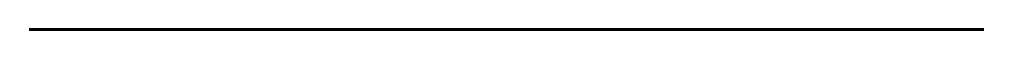
\begin{tikzpicture}
        \draw[very thick] (0,0) -- (\textwidth,0) {};
\end{tikzpicture}\FloatBarrier\parindent 0pt
\bfseries {\huge \sc{A PERFORMANCE PORTABLE CHARGE CONSERVING FDTD IMPLEMENTATION}}
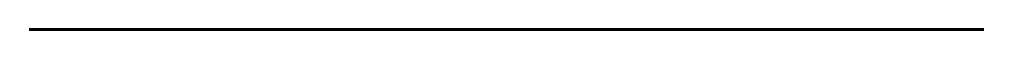
\begin{tikzpicture}
        \draw[very thick] (0,0) -- (\textwidth,0) {};
\end{tikzpicture}}
\author{
        \textsc{{{\LARGE Master Thesis}}} \\[5pt]
        \small in High Energy Physics  \\[5pt]
        \small Department of Physics \\[5pt] \small ETH Zurich \vspace{0.4cm} \\[0.2in]
        \\ \small written by \\[5pt]
        %\small \sc{BSc ETH xxx} \\
        \sc{Manuel Winkler} \\ 
        \vspace{1cm} \\
        \small supervised by \\[5pt]
        Dr.\ A.\ Adelmann (ETH)\\
		\vspace{0.5cm} \\
        \small scientific advisers \\[5pt]
        Sonali Mayani \\
        \vspace{1.5cm} \\
        \today
}
\date{}
% \clearpage
\maketitle
\thispagestyle{empty}
\end{titlepage}

\setcounter{page}{0}  % set page number -> such that table of contents is first page

%%%%%%%%%%%%%%%%%%%%%%%%%%%%%%%%%%%%%%%%%%%%%%%%%%%%%%%%%%%%%%%%%%%%%%%%%%%%%%%%%%%%%%%%%%%%%%%%%%%%%%%%%%%%%%%%%%%%%%%%%
% ABSTRACT
%%%%%%%%%%%%%%%%%%%%%%%%%%%%%%%%%%%%%%%%%%%%%%%%%%%%%%%%%%%%%%%%%%%%%%%%%%%%%%%%%%%%%%%%%%%%%%%%%%%%%%%%%%%%%%%%%%%%%%%%%

\begin{abstract}
  We implement a Finite Difference Time Domain and Particle-in-Cell solver to simulate the electromagnetic interaction processes between charged particles in strong and rapidly changing electromagnetic external fields. We aim to use Nonstandard Finite-Difference schemes to update the electromagnetic fields and a Boris-pusher to update the particles. Finally, we aim to demonstrate its correctness by reproducing results of the simulation of an infrared free electron laser known from literature. 
\end{abstract}

%%%%%%%%%%%%%%%%%%%%%%%%%%%%%%%%%%%%%%%%%%%%%%%%%%%%%%%%%%%%%%%%%%%%%%%%%%%%%%%%%%%%%%%%%%%%%%%%%%%%%%%%%%%%%%%%%%%%%%%%
% TABLE OF CONTENTS
%%%%%%%%%%%%%%%%%%%%%%%%%%%%%%%%%%%%%%%%%%%%%%%%%%%%%%%%%%%%%%%%%%%%%%%%%%%%%%%%%%%%%%%%%%%%%%%%%%%%%%%%%%%%%%%%%%%%%%%%
\newpage
\pagenumbering{roman}
\tableofcontents


% 27.08.2015, http://tex.stackexchange.com/questions/11579/captions-for-figures-in-listoffigures

% 27.08.2015, https://www.sharelatex.com/learn/Lists_of_tables_and_figures
%\listoffigures 
%\listoftables
%\lstlistoflistings
% 06.09.2015, http://tex.stackexchange.com/questions/165903/optional-caption-in-listings-for-listoflistings

%\listofmyoutputs

\newpage
\pagenumbering{arabic}

%%%%%%%%%%%%%%%%%%%%%%%%%%%%%%%%%%%%%%%%%%%%%%%%%%%%%%%%%%%%%%%%%%%%%%%%%%
\chapter{Introduction}

\section{Dimension analysis}
In order to simplify every equation in classical and quantum electrodynamics, we use aim to use a set of basis units such that the involved constants $c$, $\hbar$, $\epsilon_0$ and $mu_0$ are all equal to one. All the code described and written in \ref{discretization} and \ref{appendix} is implemented using natural units, outlined in Section \ref{scaled_planck_units}. Still, all formulae presented in this report are correct for any unit basis.

One problem arises with the use of Planck units is that many real-world quantities do not fit into a C++ `float`, representing a 32-bit floating point number. For example, with the maximum value representable in a `float` being $\approx 3.4 \cdot 10^{38}$, it is not possible to represent even one second in Planck times, which would be larger than $10^{43}$. To keep 32 bit floats an option we derive set of scaled Planck units in Section \ref{scpunits}. 
\subsection{Planck units}
\textbf{Standard Planck units} \label{scaled_planck_units}
\\
The way Planck units are usually defined \cite{planckunits}  is by setting the five fundamental constants \begin{align*} \hbar = 4\pi \epsilon_0 = c = k_B = G = 1 \end{align*}
$k_b$ and G are completely irrelevant for our problem. However, one could also pick the vacuum permittivity $\epsilon_0$ itself as 1. Therefore, this already creates two ways to define the Planck units:

\begin{align*}
  \begin{cases}
      4 \pi \epsilon_0 = 1 &\iff q_P = 11.7062371 e \text{  (Gaussian normalization)} \\
      \epsilon_0 = 1 &\iff q_P = \frac{11.7062371}{\sqrt{4 \pi}} e = 3.3022685 e
  \end{cases}
\end{align*}
 The other three Planck base units are not affected by this choice. The Planck power $\mathrm{P}_P$ for example is unaffected since the Planck voltage and Planck current are scaled in opposite directions.

We will be using Planck units with $\epsilon_0 = 1$.
\subsubsection{Scaled Planck units} \label{scpunits}

Since in our application, $G$ is of no interest, scaling the Planck units by a factor of $\\alpha$, conserving $\hbar = \epsilon_0 = c = 1$ is a good way to keep the numbers appearing in the simulation closer to 1. We denote the \textit{dimensionality} vector of a quantity $S$ as follows: $ \mathbf{D}_S = \begin{bmatrix}L_S \\ M_S \\ t_S \\ I_S \end{bmatrix} $ where $L, M, t, I$ denote length, mass, time and current. Such a dimensionality can also be assigned to each physical constant according to its units.
A constant $C$ with dimensionality $D_C$ will transform from a unit system $U$ to a scaled unit system $U_\alpha$ as follows:
\begin{align}
C_{U \alpha} = C_U \prod_i{\alpha_i^{-D_{C i}}} \end{align} \label{unit_scaling}
where $\alpha_i$ denotes the scale applied to the $i$-th dimension. 
As an example, consider the speed of light:
$ D_c = \begin{bmatrix}1 \\ 0 \\ -1 \\ 0 \end{bmatrix} $
If we stretch the length unit by a factor of 2 and the time by a factor of $\frac{1}{2}$
will evaluate to the following:
\begin{align*} c_{U_\alpha} &= c_U \prod_{D_c} {\alpha_i^{-D_{c i}}} \text{   with} \alpha = \begin{bmatrix}2 \\ 1 \\ \frac{1}{2} \\ 1 \end{bmatrix} \\ &= 2^{-1} \cdot \frac{1}{2}^1 = \frac{1}{4} \end{align*}
Therefore, if we pick a unit system where the length unit is two Planck lengths and the time unit is half a Planck time, the speed of light represented in those units will be 
\begin{align*} c = \frac{1}{4} \frac{\text{double Planck lengths}}{\text{half Planck times}} \end{align*} which is intuitively clear.
We can use \ref{unit_scaling} to construct a scaling vector that keeps a set of $m$ constants spanning $n$ dimensions constant.
The system of equations will be composed as follows:
\begin{align*} 
\prod_i \alpha_i^{-D_{\text{C} i}} &= 1 \ \text{   for every constant  } C \end{align*}
Let's consider the case \begin{align*} \alpha_i = \alpha^(x_i) \text{ where } x \in \mathbb{R}^+ \end{align*}
This results in the following equation for a constant $C$
\begin{align*}
\prod_{i} \alpha^{- x_i D_{C i}} &= 1
\end{align*}
Taking the logarithm with basis $\alpha$ on each side yields
\begin{align} 
    \sum_{i} - x_i D_{C_i} = 0 \\ \iff \sum_{i} x_i D_{C_i} = 0 
\end{align} \label{logtake}
This can be composed an $(m = 3, n = 4)$ linear system of equation in the case of fixating the three constants $\hbar, \varepsilon_0$ and $c$ to 1.
One useful solution of this system is the vector 
\begin{align*} 
e = \begin{bmatrix} 1 \\ -1 \\ 1 \\ -1 \end{bmatrix} 
\end{align*} 
which, given a scaling parameter $\alpha$, leads to the scaling vector 
\begin{align*} 
\mathbf{\alpha} = \begin{bmatrix} \alpha \\ \frac{1}{\alpha} \\ \alpha \\ \frac{1}{\alpha} \end{bmatrix} \\
\end{align*} 
This vector is obtained by undoing the logarithm to obtain \ref{logtake}
A good choice for the scaling factor $\alpha$ is $10^{30}$. This yields reasonable values for elementary particle mass and simulation domain extents. A list of all those conversions in `C++` can be found \href{https://gitlab.psi.ch/AMAS-students/winkler_msc/-/blob/main/experiments/cfg.hpp}{here}.
\chapter{Governing equations} \label{governing_eq}
\section{Wave equation} 
The general wave equation is as follows:
\begin{align} 
\frac{\partial^2 u}{\partial t^2} &= \Delta u + f 
\end{align}\label{wave_equation_general}
where $u$ denotes the target function and $f$ the source term.
\subsection{Maxwell} 's equations
The equations governing the electromagnetic fields are called *Maxwell's Equations*. \
\textbf{Electromagnetic form} 

\begin{align} 
\nabla \cdot  \mathbf{E} &= \rho\varepsilon_0 \\
\nabla \cdot  \mathbf{B} &= 0 \\
\nabla \times \mathbf{E} &= -\frac{\partial \mathbf{B}}{\partial t} \\
\nabla \times \mathbf{B} &= \mu_0 \mathbf{J} + 1 / c^2 \frac{\partial E}{\partial t}
\end{align} \label{em_maxwell}
\textbf{Potential form} 
%\let vpot = $vb(upright(A))^\alpha$
Define scalar and vector potential as follows:
\begin{align*}
 \nabla \times \mathrm{A} &= \mathbf{B} \\
 -\nabla \phi - \frac{\partial A}{\partial t} &= \mathbf{E}
\end{align*}
Define the four-source
\begin{align*}
 \mathbf{J}^\alpha &= \begin{bmatrix}\frac{1}{\varepsilon_0} \rho & \mu_0 \mathbf{J}_0, \mu_0  \mathbf{J}_1 & \mu_0 
 \mathbf{J}_2 \end{bmatrix}^T 
\end{align*}
and the four-potential
$ vpot = mat(phi "|", upright(A)_0, upright(A)_1, upright(A)_2)^T $
Maxwells equations can then be reduced to
\begin{align}
 \frac{1}{c^2} \frac{\partial^2 \mathbf{A}}{\partial t^2} &= \Delta \mathbf{A} + \mathbf{J}^\alpha 
\end{align} \label{potential_maxwell}

For a full derivation we refer to \cite{3A_Maxwell}.

\subsection{Boundary Conditions } \label{bconds_section}
\subsection{Factorization}
\subsection{The Dirac equation}
\subsection{Transforming the fields } \label{transformingthefields}
\section{Initial conditions}
\subsection{Electrostatic initial conditions }
\subsection{Boosted electrostatic initial conditions}
\subsection{Liénard -Wiechert potentials} \label{subsection_lienard}
\section{Lorentz Force}
\subsection{Relativistic limit } \label{relativistic_lorentz_force}
\chapter{Discretization} \label{discretization}
\section{Finite Difference Time Domain}
\subsection{FDTD Discretization}
\subsection{Accuracy Analysis } \label{accuracy_analysis}
\subsection{Numerical Dispersion}
\subsection{Boundary condition } \label{bcond_numeric}
\subsection{High frequency problems}
\section{Particle In Cell}
\subsection{Boris Pusher}
\subsection{Quantity Interpolation}
\subsection{Current deposition } \label{current_dep}
\subsection{Charge-conserving current deposition schemes}
\chapter{Simulation of Free Electron} Laser
\section{Input Parameters}
\subsection{Undulator}
\subsection{Bunch}
\subsection{Mesh}
\section{Lorentz Transform } \label{ltransform}
\subsection{Transforming the bunch } \label{bunch_transform}
\subsection{Laboratory-Bunch interactions}
\chapter{Implementation}
\section{Programming model}
\section{Threads}
\section{Ranks}
\section{Cuda } \label{cuda_section}
\subsection{Instructional Throughput}
\subsection{Memory Types}
\section{Performance}
\subsection{Memory Locality}
\subsection{Memory footprint}
\section{Numerically Stable Reductions}
\chapter{Results}
\section{Source-free Plane Wave}
\section{Source terms}
\subsection{Gauss 's Law}
\subsection{Ampere 's Law}
\subsection{Radiation sampling}
\section{Free Electron Laser (Infrared)}
\subsection{Forward radiation}
\section{Scaling}
\subsection{Weak scaling } \label{weak_scaling_subsection}
\subsection{Strong scaling } \label{strong_scaling_subsection}
\chapter{Conclusion}
\section{Achieved Goals}
\section{Further Research}
\chapter{Appendix} <appendix>
\section{Second order ABC edge implementation } \label{abc2_edge_implementation}
\section{Second order boundary condition corners }
\section{Rendering}
\subsection{Projective Geometry}
\subsection{Framebuffer Reduction}
\bibliography{report.bib}
\includepdf[pages={16-}]{report.pdf}
\end{document}

This can be composed an $(m = 3, n = 4)$ linear system of equation in the case of fixating the three constants $hbar$, \varepsilon_0$ and $c$ to 1:
\grid(columns: (1fr, 0.2fr, 1fr), rows: (6em))[
  \block(width: 100%, height:100%, radius:10pt, stroke: red, inset:5pt)[
    \align(horizon)[$ mat(&2, &1, -&1, &0; -&3,-&1, &4, &2;&1,&0,-&1,&0) vec(x_1,x_2,x_3,x_4) &= vec(0,0,0) $]
  ]
\nextitem
  \block(width: 100%, height: 100%)[
    \place(dx: 5%, dy: 50%, line(length: 90%, stroke:gradient.linear(red, green) + 2pt))
    \place(
      polygon(fill:gradient.linear(red, green),
        (80%,40%),
        (97%,50%),
        (80%,60%),
      )
    )
  ]
\nextitem
  \block(width: 100%, height:100%, radius:10pt, stroke: green, inset:5pt)[
    \align(horizon)[$ A vec(-&x,&x,-&x,&x) &= vb(0), x in bb(R) $]
  ]
]
One useful solution of this system is the vector $ e &= vec(&1,-&1,&1,-&1) $ which, given a scaling parameter $\alpha$, leads to the scaling vector $ vb(\alpha) = vec(\alpha, 1/\alpha,\alpha,1/\alpha) $ This vector is obtained by undoing the logarithm to obtain \ref{logtake}.
\block(breakable: false)[
  \show math.equation: set text(0.8em)
  \figure(table(align: horizon + center, fill: (i, j) => {if j == 0{rgb("aaaaff")} else if calc.rem(j,2) == 0{rgb("ffffff")} else{rgb("abc")}}, stroke: 1pt, columns: (1fr,1fr), rows: 2.6em)[
    \textbf{Quantity}
  \nextitem
    \textbf{Value}
  \nextitem 
    \textbf{Scaled Planck length}
  \nextitem
    $ \alpha dot l_P $
  \nextitem
    \textbf{Scaled Planck mass}
  \nextitem
    $ m_P / \alpha $
  \nextitem
    \textbf{Scaled Planck time}
  \nextitem
    $ \alpha dot t_P $
  \nextitem
    \textbf{Scaled Planck force}
  \nextitem
    $ F_P / (\alpha^2) &= (1.210 dot 10^44) / \alpha^2 $
  \nextitem
    \textbf{Scaled Planck current}
  \nextitem
    $ I_P / \alpha = (9.813 dot 10^24)/\alpha upright(A) $
  \nextitem
    \textbf{Scaled Planck charge}
  \nextitem
    $ q_P  = \str((11.71 / calc.sqrt(4 * calc.pi))).slice(0,5) e $
  \nextitem
    \textbf{Scaled Planck velocity}
  \nextitem
    $ v_P = c = l_P / t_P $
  \nextitem
    \text(0.8em)[\textbf{Scaled Planck magnetic flux density}]
  \nextitem
    $ Phi_P / \alpha^2 = (7.630 dot 10^53)/\alpha^2 upright(T) $
  \nextitem
    \text(0.8em)[\textbf{Scaled Planck electric strength}]
  \nextitem
    $ E_P / \alpha^2 = (2.287 dot 10^62 )/\alpha^2 space upright(V/m) $
  \nextitem
  /*  \text(0.9em)[\textbf{Scaled power density}]
  \nextitem
    $ P_D_P / \alpha^4 = (1.389 dot 10^122) / \alpha^4 upright(W/(\h(0.2em)m^2)) $
  \nextitem*/
    \text(1em)[\textbf{Scaled power}]
  \nextitem
    $ P_P / \alpha^2 = (3.628 dot 10^52) / \alpha^2 upright(W) $
  \nextitem
    \text(1em)[\textbf{Scaled power density}]
  \nextitem
    $ P_P / \alpha^2 = (1.389 dot 10^122) / \alpha^4 upright(W/m^2) $
  ], caption: "Scaled Planck units") \label{scaled_planck_units}
] 
A good choice for the scaling factor $\alpha$ is $10^{30}$. This yields reasonable values for elementary particle mass and simulation domain extents. A list of all those conversions in `C++` can be found \link("https://gitlab.psi.ch/AMAS-students/winkler_msc/-/blob/main/experiments/cfg.hpp")[\text(blue)[\textbf{here}]].
\chapter{Governing equations} \label{governing_eq}
\section{Wave equation} 
The general wave equation is as follows:
\NE[$ pdv(u, t, 2) &= laplace u + f $ \label{wave_equation_general}]
where $u$ denotes the target function and $f$ the source term.
\subsection{Maxwell} 's equations
The equations governing the electromagnetic fields are called *Maxwell's Equations*. \
\textbf{Electromagnetic form} 
\NE[
$ &nabla \h(0.5em) dot &vb(upright(E)) &&&= rho\varepsilon_0 \
  &nabla \h(0.5em) dot &vb(upright(B)) &&&= 0 \
&nabla times &vb(upright(E)) &&&= -pdv(B, t) \
&nabla times &vb(upright(B)) &&&= mu_0 vb(upright(J)) + 1 / c^2 pdv(E, t) $ \label{em_maxwell}]
\textbf{Potential form} 
\let vpot = $vb(upright(A))^\alpha$
Define scalar and vector potential as follows:
$ nabla times A = vb(upright(B)) $
$ -nabla phi - pdv(A, t) = vb(upright(E)) $

Define the four-source
$ vb(upright(J))^\alpha &= mat(lr(display(1\varepsilon_0) rho space "|"), mu_0 vb(upright(J))_0, mu_0  vb(upright(J))_1, mu_0 
 vb(upright(J))_2)^T $
and the four-potential
$ vpot = mat(phi "|", upright(A)_0, upright(A)_1, upright(A)_2)^T $
Maxwells equations can then be reduced to

\NE[$ 1/c^2 pdv(vpot, t, 2) = laplace vpot + vb(upright(J))^\alpha $ \label{potential_maxwell}]

For a full derivation we refer to \ref{}3A_Maxwell.

\subsection{Boundary Conditions } \label{bconds_section}
The evolution of values of $vpot$ on the domain boundary can be parametrized in several ways. The simplest equation to parametrize the boundary is to lock it to the constant value 0, known as \textbf{Dirichlet Boundary conditions}: \NE[$ vpot(x) = 0 space forall x in partial Omega $ \label{dirichlet_bc}]
Alternatively, the outward gradient can be fixed to zero, leading to *Neumann boundary conditions: *
$ pdv(vpot, vb(n))(x) &= 0 space forall x in partial Omega $
However, for simulation taking place in open space, the the boundary conditions usually of interest are absorbing boundary conditions. Absorbing boundary conditions are equivalent to an "open" domain boundary -- where outgoing waves simply leave the domain. As it turns out, those are the hardest to derive and implement numerically.  
\subsection{Factorization} 
To get an intuitive sense on absorbing boundary conditions, consider the one-dimensional wave equation \NE[$ pdv(u,t,2) - c^2pdv(u, x, 2) = 0 $ \label{wave_1d} ] defined on an interval $[0,L]$. 
This equation can be factorized into two factors:
\NE[$ (c pdv(, x) + pdv(, t))(c pdv(, x) - pdv(, t))u = 0 $ \label{wave_factorization} ]
Therefore, any $u$ that satisfies either of the unidirectional advection equations $ &(c pdv(, x) - pdv(, t))u^- &= 0 \ &(c pdv(, x) + pdv(, t))u^+ &= 0 $
is a solution for the wave equation, where $u^-$ describes left-moving waves and $u^+$ describes right-moving waves. As long as we can represent $u$ as a superposition $ u = u^+ + u^-, $
$u$ satisfies \ref{wave_}1d. As an example, consider the \ref{wave_}1d with initial conditions: 
$
  u(x=0,t=0) &= f(x) \ accent(u,dot)(x=0,t=0) &= g(x)
$
\let up = $u^+$
\let um = $u^-$
\let iff = $<==>$
By definition we have $ pdv(u^plus.minus, t) = minus.plus c pdv(u^plus.minus, x), $
leading to two conditions. Since
$ pdv(,t)lr(size: \2.2em, (up + um)) = g $

$ <==> cases(display(c pdv(,x))&lr(size: \2.2em, (um - up)) = g, &lr(size: \2.2em, (um + up)) = f iff up = f - um) $

\show math.chi : it => {move(dy: -0.2em, it)}
Manipulating the terms and replacing $up$ we obtain
$ c pdv(, x)(2 um - f) &= g iff c pdv(,x)um = 1/2 (g + pdv(,x)f) $
\NE[$ iff um(t = 0,x) &= 1/(2 c) lr(size: \2.3em, (integral_(L_"lower")^x g(chi) upright(d)chi + f(x))) $ \label{split_into_ump}]
where the $L_"lower"$ denotes the lower limit of our domain of definition. \ref{split_into_ump} therefore describes a conversion from a state of the wave equation represented as $u$ and its temporal derivative $accent(u,dot)$ to a representation as a left and a right moving part $um$ and $up$. The three most important special cases are 
\context{
let wi = measure($display(f(x)/2)$).width
let he = measure($display(f(x)/2)$).height
//let bbox(it) = box(width: wi, height: he, it)[\it]
$ vec(u, accent(u, dot))_(t = 0) &= vec(\hide[$-$] &f, &0) \h(1.4em) &&==> \h(1.4em) vec(up, um) = vec(display(f/2), display(f/2)) \ 
  vec(u, accent(u, dot))_(t = 0) &= vec(\hide[$-$] &f, &c f) \h(1.4em) &&==> \h(1.4em) vec(up, um) = vec(f,0) \ 
  vec(u, accent(u, dot))_(t = 0) &= vec(&f, -&c f) \h(1.4em) &&==> \h(1.4em) vec(up, um) = vec(0,f) $ 
} \
\textbf{Complex representation } \label{cwave}
\let uc = $vb(upright(U))$
We can represent the state of the wave equation in the a complex form. We define the $uc$ and its temporal and spatial derivatives as follows:
\block(breakable: false)[
$ vb(upright(U))(x, t) &= pdv(,x)u(x, t) + ii \h(0.1em) pdv(,t) (x, t) $

$ vb(upright(U))_(k, omega) = e^(ii(k x - omega t)) $
\[
  \show math.equation: it => {math.display(it)} 
\table(rows: 3em, align: center + horizon, columns: (1fr, 1fr, 1fr, 1fr), fill: (i,j) => {
  if (j > 0){rgb("ddffdd")}
  else{rgb("ffffcc")}
})[$pdv(, t)$\nextitem$pdv(, x)$\nextitem$pdv(, t, 2)$\nextitem$pdv(, x, 2)$\nextitem
  $ - ii omega uc $
\nextitem
  $ ii k uc $
\nextitem
  $ - omega^2 uc $
\nextitem
  $ -k^2 uc $
]
]]
Notice that inserting the second derivatives into the wave equation (\ref{wave_equation_general}) we obtain $ omega^2 = c^2 k^2 iff omega = plus.minus c k, $ 
giving us a nice representation of right and left travelling waves, determined by whether $omega$ and $k$ have different signs. A fourier transform of $upright(bold(U))$ yields the amplitude of every right and left moving mode.
\ 
\textbf{Boundaries } 
Back to a purely real $u(x, t) in RR times RR -> RR$: If we guarantee $ (pdv(, x) - pdv(, t)) u &= lr(0|, size: \2em)_(x = 0) \ (pdv(, x) + pdv(, t)) u &= lr(0|, size: \2em)_(x = L) $
waves colliding with the boundary will be perfectly absorbed. For multidimensional absorbing boundary conditions, consider the derivation in \ref{mittra_abc}:
\NE[$ (pdv(, x) - sqrt(1/c^2 pdv(, t, 2) - pdv(, y, 2) - pdv(, z, 2))) = lr(0 " "|, size: \3.1em)_(x = 0) $ \label{perfect_abc}]
\ref{perfect_abc} describes a perfectly absorbing boundary in $x= 0$, however evaluating the square root is not possible using local stencils, because it is a global operator. For a thorough explanation on global operators, the reader is referred to \ref{mittra_abc}. It is clear that \ref{perfect_abc} is the three-dimensional equivalent of \ref{wave_factorization}, since clearly \NE[$ (pdv(, x) - sqrt(1/c^2 pdv(, t, 2) - pdv(, y, 2) - pdv(, z, 2)))(pdv(, x) + sqrt(1/c^2 pdv(, t, 2) - pdv(, y, 2) - pdv(, z, 2))) = laplace + pdv(,t,2) = square $ \label{xfactor}]
The Taylor expansions of \ref{perfect_abc} to first and second order are called Mur's First and Second order Absorbing Boundary Conditions \ref{Mur}1981. The expansions are as follows: 
\NE[$ 
      plus.minus pdv(u, x, t) - 1/c &pdv(u, t, 2)                                       &&= 0 " (first order)" , \
      plus.minus pdv(u, x, t) - 1/c &pdv(u, t, 2) - c/2 pdv(u, y, 2) - c/2 pdv(u, z, 2) &&= 0 " (second order)"
$ \label{mur_abc}]
These are two expressions that only depend on derivatives that are approximatable by stencils. It should be noted that the second order variant from \ref{mur_abc} is equivalent to 
$ plus.minus pdv(u, x) - 1/c pdv(u, t) = 0 $ which is a particularly easy expression to discretize, see \ref{abc_firstorder_discretizations}.
\let EF = $vb(upright(E))$
\let BF = $vb(upright(B))$
\subsection{The Dirac equation} 
As of \ref{xfactor}, we can construct a real factorization for the three-dimensional wave equation. Constructing a real (or even complex) factorization of the three-dimensional wave equation $ lr((1/c^2pdv(,t,2) - pdv(,x,2) - pdv(,y,2) - pdv(,z,2)))u = 0 = square u $ is not possible. We can however simply write down the equation and then use the desired result to define our coefficients:
\[
  \[$ lr((gamma_0 1/c pdv(,t) + gamma_1 pdv(,x) + gamma_2 pdv(,y) + gamma_3 pdv(,z)))lr((gamma_0 1/c pdv(,t) + gamma_1 pdv(,x) + gamma_2 pdv(,y) + gamma_3 pdv(,z))) =^display(!) square $]
  Expanding the terms, we obtain a condition for $gamma_i$
  $ gamma_i gamma_j + gamma_j gamma_i &= cases(2 " if " i = j, 0 " otherwise") $
  These conditions are fulfilled by the Dirac-matrices $gamma_(1..4)$ \ref{macfarlane} \ref{collas}2019dirac.
] \
\textbf{Energy conservation} 
\linebreak
The source-free wave equation  conserves the energy contained in $vpot$. The energy density of $vpot$ is obtained through the electromagnetic energy-stress tensor derived in \ref{Misner}1973:
\NE[
$ T_(mu nu) &= T^(mu nu) = F^(mu \alpha) F^(nu)_\alpha - 1/4 eta ^ (mu nu) F_(\alpha \beta) F^(\alpha \beta) $ \label{energy_stress} where $F_(mu nu)$ is the Faraday Tensor and $eta^(mu nu)$ is the Minkowski metric: 
$ eta^(mu nu) = mat(-1,0,0,0;0,1,0,0;0,0,1,0;0,0,0,1) $
and \
\[$ F^(mu nu) = partial^mu vb(upright(A))^nu - partial^mu vb(upright(A))^nu. $] \label{faraday}]

\textbf{Energy Density} 
\ The energy density per unit volume is given by $ T_00 = 1/2\varepsilon.alt_0 EF^2 + 1/mu_0 BF^2) $ \
Evaluated in SI units this yields an energy density of units $upright(J/m^3) = upright(N/m^2) = "Pa"$. 
\
\textbf{Energy Flux} 
\ The first row (or column, since $T^(mu nu) = T^(nu mu)$) of $T^(mu nu)$ reads
$ mat(T_00,display(1/c) S_x,display(1/c) S_y,display(1/c) S_z) $ where
\NE[$ S = 1/mu_0 (EF times BF) $ \label{poynting_vector}] denotes the \textbf{Poynting Vector}.
The unit of $S$ is $upright(W/m^2)$, therefore the unit of $1/c S$ is $upright(J/m^3)$.

We can write the following conservation law:
\NE[$ bold(nabla) dot S = -dd(cal(U))/dd(t) " where " cal(U) = T_00 $ \label{conservation_law_differential}]
As always, we can rewrite \ref{conservation_law_differential} in integral form: 
\NE[$ dd(integral_Omega cal(U))/dd(t) = integral_(partial Omega) S dot dd(va(n)) $ \label{conservation_law_integral}]
Verifying if \ref{conservation_law_integral} is fulfilled at all times is numerically trivial and a good sanity check on a FDTD implementation. //One test that performs such a surface integral is described im\ref{synchrotron_test}.
\subsection{Transforming the fields } \label{transformingthefields}
The electric and magnetic field are transformed from laboratory to bunch coordinates as seen in \ref{daniel}1997elektrodynamik:
\NE[$ vb(upright(E))_"bunch" &= gamma lr(size: \2em,(vb(upright(E))_"lab" + vb(v) times vb(upright(B))_"lab"&&)) - (gamma - 1)(vb(upright(E))_"lab" dot accent(vb(v), hat))accent(vb(v), hat) \
 vb(upright(B))_"bunch" &= gamma (vb(upright(B))_"lab" - (vb(v) times vb(upright(E))_"lab")/c^2&&) - (gamma - 1)(vb(upright(B))_"lab" dot accent(vb(v), hat))accent(vb(v), hat) $ \label{eb_transform}] 
 where $ &vb(v) " denotes the frames relative velocity" \ &vb(accent(v, hat)) " denotes the normalized velocity " vb(v)/(||vb(v)||) \ "and " &gamma " denotes the corresponding lorentz factor " 1/sqrt(1 - display((||v||_2^2)/c^2)) $
Furthermore, for the special case that $vb(v) = vec(0,0,c \beta_z)$ the relativistic doppler effect is described by the formula \NE[$ lambda_"lab" &= lambda_"bunch" sqrt((1 - \beta_z) / (1 + \beta_z)) \ &=  1/(gamma(1 - \beta)) lambda_"bunch" $ \label{doppler}]
whereas the poynting vector transforms as follows
\NE[$ EF_"lab" times BF_"lab" = (1 + \beta_z)/(1 - \beta_z)lr(size: \2.3em, (EF_"bunch" times BF_"bunch")) $ \label{poynting_lorentztransform}]
\ref{doppler} and \ref{poynting_lorentztransform} are different in that the scaling factor of \ref{doppler} is the root of the scaling factor of \ref{poynting_lorentztransform}. This is due to the fact that \ref{poynting_lorentztransform} doesn't take into account that a stationary detector in one frame is not stationary in another. For a thorough derivation on the radiation passing through a screen measured in different inertial frames (or the radiation reflected off it), the reader is referred to \linkbox(cite(<taflove1995>, style: "the-institution-of-engineering-and-technology", supplement: ", Section 10.9.2")).
\section{Initial conditions} 
\subsection{Electrostatic initial conditions } 
If an initial charge distribution is known and the initial current distribution is zero, simply solving a poisson equation \NE[$ -laplace phi = rho /\varepsilon_0 $\label{ic_electrostatic}] will yield a suitable $ vpot = vec(phi, upright(A)_0, upright(A)_1, upright(A)_2), upright(A) = vb(0) $ 
Several approaches on fast poisson solvers exist \ref{witch} \ref{ippl}.
\subsection{Boosted electrostatic initial conditions} 
If all particles are moving with the exact same speed, one can compute an initial condition in an exactly comoving frame according to \ref{ic_electrostatic}, and then use \ref{eb_transform} to transform them back to the oroginal frame. Analogous to the explanation in paragraph \ref{time_correction}, we end up with grid values captured at different points in time. This artifact is usually ignored \ref{conv_arnau}.
\subsection{Lienard} -Wiechert potentials \label{subsection_lienard}
A generalized and classically perfect condition for the electromagnetic fields imposed by a moving charge is given by the Lienard-Wiechert Potentials \ref{lienard_ref}:
For a particle with a trajectory $va(R)(t)$ and velocity
$ va(\beta)(t) = va(R)(t), $
only an implicit equation for the scalar potential at a measurement point $va(r)$ can be stated:
\NE[
  $ Phi(va(r), t) = q/(4 pi\varepsilon_0(1 - va(\beta)(t_"ret") dot va(n))|r - va(R)(t_"ret")|) $ \label{lienard_wiechert_potential}
  and also the vector potential
  $ A(va(r), t) = va(\beta)(t_"ret")/c phi(va(r), t), $ \label{lienard_wiechert_vpot}
  where
  $ t_"ret" (t, va(r)) &= t - 1/c|va(r) - va(R)(t_"ret")| $ \label{tret_relation}
  and $ va(n) = (va(r) - va(R))/(|va(r) - va(R)|) $
  For a proof as to why \ref{tret_relation} always has a unique solution, the reader is referred to \ref{lienard_deriv}.
  \
]
For the special case of a straight line
$ va(R)(t) = vec(0,0,c \beta t), $
we can solve the value of $t_"ret" (va(r))$ analytically. 
\NE[
  \show math.dot: none
  //\set text(size: 0.85em)
  $ t_"ret"(t, va(r)) &= (c dot t - \beta dot r_2 - sqrt(\beta^2 dot c^2 dot t^2 - \beta^2 dot r_0^2 - \beta^2 dot r_1^2 - 2 dot \beta dot c dot r_2 dot t + r_0^2 + r_1^2 + r_2^2)) / (c dot (1 - \beta^2)) $ \label{tret_straightline_solution} ]
We can insert the analytical solution \ref{tret_straightline_solution} into \ref{lienard_wiechert_potential} and \ref{lienard_wiechert_vpot} to obtain a generally correct expression for $vpot$ at any location. However, this can become extremely expensive to do. For a grid with resolution $N^3$ and $N_p$ particles, we have to evaluate \ref{tret_straightline_solution} $N^3 N_p$ times. For the special case that all particles share a common $va(\beta)$, we can implement an FFT-based convolution solver similar analogous to the Vico-Greengard method presented in \ref{witch}, reducing the cost to $approx (2 N)^3 log N + N_p$. For the general case, the evaluation of \ref{tret_straightline_solution}, let alone a solution for more complex trajectories, do not reduce to a convolution and are not optimizable any further.
\section{Lorentz Force} 
\subsection{Relativistic limit } \label{relativistic_lorentz_force}
\let etot = $cal(E)$
An analysis of a charged particle moving in an electromagnetic field is best done by representing it in a covariant four-momentum:

\NE[$ p^\alpha = {etot / c, gamma vb(p)} = gamma{m c, vb(p)} = (dd(x^\alpha)) / dd(tau) = m u^\alpha $ \label{relativistic_momentum_roc}]

where \etot denotes the total energy (symbol $vb(upright(E))$ is reserved for the electric field) $tau$ denotes _proper_ time and therefore \NE[$ gamma dd(tau) &= dd(t) $ \label{time_dilatation}] and $ u^\alpha &= dd(x^\alpha) / dd(tau), \ u_\alpha &= dd(x_\alpha) / dd(tau). $
\let customref(str, content) = {
  show ref: it => {(link(it.element.location(), str))}
  linkbox(content)
}
A fully relativity-compliant rate of change for $p^\alpha$ can be written with the \ref{faraday} $upright(bold(F))$ as follows

\NE[$ dd(p^\alpha) / dd(t) &= q upright(F)^(\alpha \beta) u_\beta $ \label{covariant_eom}]

Inspection of the first component of \ref{covariant_eom} yields: \ref{essentials} \NE[$ dd(etot) / dd(t) = q vb(upright(E)) dot vb(u). $ \label{energy_change}]
As a consequence, a change of energy is only possible by moving non-perpendicularly with a nonzero electric field.

Inspection of the second component of \ref{covariant_eom} yields: \ref{essentials}
$ dd(p) / dd(tau) &= q gamma [upright(EF)  + u times upright(BF)]_x $
which, due to \ref{time_dilatation} is consistent with the classical Lorentz force $ uv(F) &= q uv(E) + q uv(v) times uv(B). $
We can characterize a particle's motion in a constant external magnetic field of strength $B_0$ for two different regimens, the nonrelativistic and the relativistic one. For the nonrelativistic case we have:
$ (m_e v^2)/r &= q v B_0 \ <==> r &= (m_e v) / (q B_0), $
which is known as the synchrotron radius.
whereas for the relativistic case we have \ref{essentials} $ r = (m_e gamma v) / (q B_0). $
//It is well-known that a particle travelling along such a circular orbit continuously loses energy. 
\pagebreak
\chapter{Discretization} \label{discretization}
In order to solve \ref{em_maxwell} or \ref{potential_maxwell}, several approaches exist \ref{adi_zhenchenzhang} \ref{yee_maxwell} \ref{taflove}1995 \ref{mur_abc}. We will pursue variation of \ref{yee_maxwell} in potential form, called _Finite Difference Time Domain_, usually abbreviated with FDTD.
\section{Finite Difference Time Domain} 
In order to solve \ref{potential_maxwell} numerically, we discretize the field $vpot$ onto a grid with resolution $n_x,n_y,n_z$ and spacing $Delta_x, Delta_y, Delta_z$ in each direction. Spatial and temporal derivatives are computed with local convolutions called stencils. A finite-difference stencil is a formula used to approximate derivatives at a given position in a grid using function values sampled at finite intervals around the point of interest. The use of the word "local" is warranted since most of the time, only the 2-6 nearest samples are taken into account to approximate operators like $pdv(,x)$ or $laplace$. We use the following notation to describe a sample of $u$ in space and time:
\text(1.3em)[$ u^n_(i,j,k) $] denotes the value of $u$ at the point $ vec(i Delta x,i Delta y,i Delta z) " at time " n Delta t $
\let vpot = $vb(upright(A))$
Because both superscript and subscript indices are required, from here on the four-potential is denoted simply as \vpot. For a technical definition and introduction to stencils, the reader is referred to \ref{bthesis} and \ref{accuracy_analysis}.
\subsection{FDTD Discretization} 
\ref{potential_maxwell} is discretized as follows \ref{fallahi}2020mithra: 
\NE[
  $ pdv(vpot^n_(i,j,k), x, 2) &= (vpot^n_(i+1,j,k) - 2vpot^n_(i,j,k) + vpot^n_(i-1,j,k)) / (Delta x^2) \ 
    pdv(vpot^n_(i,j,k), y, 2) &= (vpot^n_(i,j+1,k) - 2vpot^n_(i,j,k) + vpot^n_(i,j-1,k)) / (Delta y^2) \
    pdv(vpot^n_(i,j,k), z, 2) &= (vpot^n_(i,j,k+1) - 2vpot^n_(i,j,k) + vpot^n_(i,j,k-1)) / (Delta z^2) \
    pdv(vpot^n_(i,j,k), t, 2) &= (vpot^(n+1)_(i,j,k) - 2vpot^n_(i,j,k) + vpot^(n-1)_(i,j,k)) / (Delta t^2) $ \label{fdtd_fielddiscretization}
]
We solve \ref{potential_maxwell} with the  \[\show "Eq." : "discretizations"; \ref{fdtd_fielddiscretization}] for $vpot^(n+1)_(i,j,k)$ and obtain:
\NE[
  \let ddx = $((c Delta t)/(Delta x))^2$
  \let ddy = $((c Delta t)/(Delta y))^2$
  \let ddz = $((c Delta t)/(Delta z))^2$
  \let \alpha1 = $\alpha_1$
  \let \alpha2 = $\alpha_2$
  \let \alpha4 = $\alpha_4$
  \let \alpha6 = $\alpha_6$
  \let \alpha8 = $\alpha_8$
  $ vpot^(n+1)_(i,j,k) = &- vpot^(n-1)_(i,j,k) 
  +  \alpha1 vpot^n_(i,j,k) 
  +  \alpha2 vpot^n_(i+1,j,k) 
  +  \alpha2 vpot^n_(i-1,j,k)\ 
  + &\alpha4 vpot^n_(i,j+,k) 
  +  \alpha4 vpot^n_(i,j-1,k) 
  +  \alpha6 vpot^n_(i,j,k+1) 
  +  \alpha6 vpot^n_(i,j,k-1)\
  + &\alpha8 upright(bold(J))^n_(i,j,k)
  $ \label{standard_fdtd_update}
  where
  \let \alpha1 = $2 lr((1 - ddx - ddy - ddz))$
  \let \alpha2 = $ddx$
  \let \alpha4 = $ddx$
  \let \alpha6 = $ddx$
  \let \alpha8 = $(c Delta t)^2$
  $ 
    \alpha_1 &= \alpha1 \
    \alpha_2 &= \alpha2 \
    \alpha_4 &= \alpha4 \
    \alpha_6 &= \alpha6 \
    \alpha_8 &= \alpha8 
  $ \label{fdtd_weights}
  The term $upright(bold(J))^n_(i,j,k)$ represents the source term at timestep $n Delta t$:
  $ upright(bold(J))^n_(i,j,k) = vec(display(rho^n_(i,j,k) /\varepsilon_0), \line(stroke: black), mu_0 J^n_(x,i,j,k), mu_0 J_(y,i,j,k), mu_0 J_(z,i,j,k)) $ \label{discretized_sourceterm}
  How the the values for $rho$ and $J$ are obtained for \ref{discretized_sourceterm} is described in \[
    \show ref: it => {link(it.element.location(), "Particle to grid interpolation.")}
    \ref{particle_to_grid}
  ]
  
]
\subsection{Accuracy Analysis } \label{accuracy_analysis}
In order to analyze how closely a stencil approximates a given derivative, consider the Taylor Expansion of an arbitrary analytical function $f$ at $0$:
$ f(x) = sum_(k=0)^oo (upright(d)^k f(0)) / dd(x)^k x^k / k! $
The evaluation of the k-th term on a gridpoint $i Delta x, i in bb(Z)$ is
$ F^k_i = (upright(d)^k f(0)) / dd(x)^k (i Delta x)^k / k! $
We define the $p$-th derivative-basis vector $b_p^n$ as follows $ b_p^n &= vec(cases(display((upright(d)^n f(0))/dd(x)^n " if " p=n), display(0 " otherwise")), dots.v) $
Therefore, $F_i^k$ expressed in basis $b_p^n$ is $ bb(F)_i^k = (i Delta x)^k / k! $
To obtain the weight vector $w$ for the $n$-th derivative the following linear system of equations has to be solved \ref{sadr}: \NE[$ bb(F)_i^k w^i &= e_n \ e_n^i &= vec(cases(1 " if " i = n, 0 " otherwise "), dots.v) $
\label{stencil_lse}] 
Solving \ref{stencil_lse} amounts to solving a linear system of equations. As an example, let's derive a first-order accurate stencil for the second derivative using three points ${-Delta x, 0, Delta x}$.
The linear system of equations that we obtain is
\block(width:100%, stroke: 0pt, height:auto)[
  $ mat(1,1,1;-Delta x,0,Delta x;\place(line(start:(-2%,0.72em), end:(29%,0.72em), stroke:red)) (Delta x^2)/2,0,(Delta x^2)/2;-(Delta x^3)/6,0,(Delta x^3)/6;dots.v,dots.v,dots.v) \move(dy: -0.7cm,$ vec(w_1,w_2,w_3) $) = vec(0,0,1,0, dots.v) $
]
As indicated by the red line, we can only guarantee a solution for the top three entries. The solution obtained is $ vec(w_1, w_2, w_3) = 1/(Delta x^2)vec(&1, -&2, &1) $
However, due to a fortunate coincidence, our solution also happens to satisfy the fourth equation. We therefore obtain second order accuracy "for free", since the linear combination of expansion is as follows:
$ Delta x^2 lr((0 + 0 + (upright(d)^2 f)/dd(x) + 0 + sum_(i = 4)^oo Delta x^(i - 2)(upright(d)^i f) / (upright(d)x^i) )) $
The $0$ coefficient for the cubic term causes the coincidental increase in accuracy from order 1 to order 2.
\subsection{Numerical Dispersion} 
One effect of the inaccuracy derived in \ref{accuracy_analysis} is a spurious slowing effect on high-frequency waves. The analysis of a plane wave parameterized by 
$ u(x, t) = e^(cal(i)(vb(k) dot vb(x) - omega t)) $ travelling through a discretized domain gives insight into why this slowdown happens and eventually yield a relation between the temporal frequency $omega$ and the spatial wavenumber $k$ \
\textbf{Numerical Dispersion} 
Consider the source-free 1-Dimensional FDTD update:
\NE[$ (u^(n+1)_(i) - 2 u^n_(i) + u^(n-1)_(i))/(Delta t ^2) = 1/c^2 (u^(n)_(i+1) - 2 u^n_(i) + u^(n)_(i-1))/(Delta x^2) $ \label{disp1}]
As described in \ref{taflove}1995, we replace all occurrences of $u$ with a plane-wave with frequency $omega$:
\[
  
  \let dt = $Delta t$
  \let dx = $Delta x$
  \let w = $omega$
  \[\show "w" : $omega$
  
  $ u^n_i = e^display(ii(k (i Delta x) - omega (n Delta t))) $
  where $ii$ denotes the imaginary unit. \
  After some manipulation an the usage of the identity $ e^(ii phi) + e^(-ii phi) = 2 cos(phi) $ \ref{disp}1 becomes
  $ 2 cos(dt w)/(c dt^2) -2 cos(dx k)/dx^2 + 2/dx^2 - 2/(c dt^2) &= 0 \
    <==> cos(dx k) (c dt^2)/(dx^2) - (c dt^2)/dx^2 + 1 &= cos(dt w) $
  ]
  We solve for $k$ following the simplifications outlined in \linkbox(cite(<taflove1995>, style: "the-institution-of-engineering-and-technology", supplement: ", Section 2.6.3")) and obtain: \NE[
    $ k = 1/(Delta x) cos^(-1)lr((1 + (dx / (c dt))^2 lr((cos(omega Delta t)-1)))) $ 
  \label{dispersion_relation}]
  \ref{dispersion_relation} is the dispersion relation for the 1D FDTD scheme: it relates the dependence of $k$ on $c$ and $omega$ with respect to the domain discretization parameters $Delta x$ and $Delta t$. Comparing it to the dispersion relation of an electromagnetic wave travelling in vacuum:
  $ k = omega / c $
  we notice that this linear dependence is only fulfilled for $Delta x = c Delta t$, since in that case \ref{dispersion_relation} simplifies to
  $ k = 1/(Delta x) cos^(-1)lr(size: \3em, (cos(omega /c Delta x))) = omega / c $
  Unfortunately, setting $Delta x = c Delta t$ is only possible for one dimension, due to the CFL condition which is derived abundantly in literature \ref{cfl_condition} \ref{fallahi}2020mithra \ref{taflove}1995:
  \NE[$ Delta t <= 1/(c sqrt(
      display(sum_i^N) display((1/(Delta x_i)))^2
    )
  ) $ \label{CFL}]
  where $N$ is the number of dimensions of the simulation. Evidently, $Delta x = c Delta t$ is only satisfiable for $N=1$. For $N=3$, we have $ Delta t <= 1/sqrt(3) Delta x approx 0.57 Delta x $
]
However, dispersion can be nullified for one direction. Following some steps out of \ref{fallahi}2020mithra, we obtain a modified version of the FDTD update equation \ref{standard_fdtd_update}:
\NE[
  \set text(0.8em)
  \show math.psi: vpot
$ 
psi_(i,j,k)^(n+1) &= -psi_(i,j,k)^(n-1)+ \alpha'_1 psi_(i,j,k)^n \
&+ \alpha'_2 ( cal(A) psi_(i+1,j,k-1)^n + (1-2cal(A)) psi_(i+1,j,k)^n &&&+ cal(A) psi_(i+1,j,k+1)^n &&&&) \ 
&+ \alpha'_3 ( cal(A) psi_(i-1,j,k-1)^n + (1-2cal(A)) psi_(i-1,j,k)^n &&&+ cal(A) psi_(i-1,j,k+1)^n &&&&) \ 
&+ \alpha'_4 ( cal(A) psi_(i,j+1,k-1)^n + (1-2cal(A)) psi_(i,j+1,k)^n &&&+ cal(A) psi_(i,j+1,k+1)^n &&&&) \
&+ \alpha'_5 ( cal(A) psi_(i,j-1,k-1)^n + (1-2cal(A)) psi_(i,j-1,k)^n &&&+ cal(A) psi_(i,j-1,k+1)^n &&&&) \
&+ \alpha'_6 psi_(i,j,k+1)^n + \alpha'_7 psi_(i,j,k-1)^n + \alpha'_8 vb(upright(J))_(i,j,k)^n
 $ \label{nsfd_update}
]
Where $\alpha'_i$ are obtained as follows:
\NE[$
\alpha'_1&=2 lr((1-(1-2 cal(A))((c Delta t)/(Delta x))^2-(1-2 cal(A))((c Delta t)/(Delta y))^2 - ((c Delta t)/(Delta z))^2 )) \
\alpha'_2&=\alpha'_3=((c Delta t)/(Delta x))^2 \
\alpha'_4&=\alpha'_5=((c Delta t)/(Delta y))^2 \
\alpha'_6&=\alpha'_7=((c Delta t)/(Delta z))^2 - 2 cal(A) ((c Delta t)/(Delta x))^2 - 2 cal(A) ((c Delta t)/(Delta y))^2 \
\alpha'_8&=(c Delta t )^2 \
$ \label{nsfd_weights}]
\[
\let frac1 = $(Delta z) / (Delta x)$
\let frac2 = $(Delta z) / (Delta y)$
\block(breakable: false)[\table(columns: 1fr, rows:(1.7cm, 2.7cm, 1.7cm, 1.7cm), align: horizon)[
  \align(center, text(1.2em, weight: 900, rgb("880000"))[\align(left)[With the following requirements:]])\nextitem

  $ cal(A) > 1/4 ", in our case: " 1/4(1 + (0.02)/((frac1)^2 + (frac2)^2)) $\nextitem
  $  Delta t = (Delta z) / c $ \nextitem
  $  (frac1)^2 + (frac2)^2 < 1 $ ]
]]
\ref{nsfd_update} and \ref{nsfd_weights} are also found in \ref{fallahi}2020mithra, with a typo corrected in the formula for $\alpha'_6$ and $\alpha'_7$


\subsection{Boundary condition } \label{bcond_numeric}
\textbf{Reflecting boundary conditions} 
If we simply lock the values on the boundary to zero as follows:
$ vpot &= vb(0) " on " partial Omega \
  vpot^(n+1)_(i,j,k) &= vb(0) " for " {i,j,k} " on the boundary" $
we obtain a boundary condition that reflects incoming waves perfectly. These boundary conditions are called Dirichlet Boundary Conditions. For simulation domains enclosed by perfect conductors this is desirable, however we also want to perform simulations in open space. \

\textbf{Absorbing boundary condtions} 
As outlined in \ref{bconds_section}, we want waves in our domain to be able to freely leave through the boundary. \
\textbf{First Order Mur Absorbing Boundary Conditions} 
\let frac(x,y) = $(\x)/(\y)$
\NE[$ pdv(vpot, vb(upright(n))) - 1/c pdv(vpot,t) &= 0 $ \label{mur_firstorder_again} ]
Let's take a look at \ref{mur_firstorder_again} on the boundary at the $x = 0$ boundary: 
$ x &= 0, vb(upright(n)) = vec(-&1,&0,&0) $ 
\NE[$ pdv(vpot, x) + 1/c pdv(vpot, t) &= 0 $ \label{abc_xboundary} ]
In order discretize \ref{abc_xboundary} with second order accuracy, we have to perform the discretization half a spatial step away from the boundary and half a timestep into the future: $ 
  lr(pdv(vpot, x) |)_(x=(Delta x)/2,t=(Delta t)/2) &approx (vpot^(n)_1   - vpot_0^n + vpot^(n+1)_1 - vpot_0^(n+1)) / (2 Delta x) 
\ lr(pdv(vpot, t) |)_(x=(Delta x)/2,t=(Delta t)/2) &approx (vpot^(n+1)_0 - vpot_0^n + vpot^(n+1)_1 - vpot_1^n)     / (2 Delta t)
$ 
Solving \ref{abc_xboundary} with these discretizations applied for $vpot_0^(n+1)$ yields \ref{mittra_abc} \ref{Mur}1981:
\[
  \let dt = $Delta t$
  \let dx = $Delta x$
  \let A00 = $vpot^n_0$
  \let A01 = $vpot^n_1$
  \let A10 = $vpot^(n+1)_0$
  \let A11 = $vpot^(n+1)_1$
  $ A10 &= (-A00 c dt + A00 dx + A01 c dt + A01 dx + A11 c dt - A11 dx)/(c dt + dx) $
]

\NE[
  \let aa = $vb(upright(A))$
  \let an = $vb(upright(A))^n$
  \let anm1 = $vb(upright(A))^(n - 1)$
$ \label{==> aa^(n+1)_0 &= aa^n_1 + (c Delta t - Delta x) / (c Delta t + Delta x) (aa^(n+1)_1 - aa^(n)_0) $ <mittras_firstorderdisc}
Where $aa_i$ represents $aa_(i,j,k)$, the transversal indices $j,k$ are dropped for brevity. It should be noted that \ref{mittras_firstorderdisc} only depends on two temporal instances of $aa$. The discretization found in \ref{fallahi}2020mithra is done differently: instead of \ref{abc_xboundary}, the following expression is used on the $x=0$ boundary:
$ pdv(vpot, x, t) + 1/c pdv(vpot, t, 2) &= 0 $ \label{fallahi_firstorder_analytical}
Following \ref{fallahi}2020mithra, \ref{fallahi_firstorder_analytical} is then discretized as follows:

$ &lr(pdv(vpot, x, t) |)_(x=(Delta x)/2, t = 0) && approx 1/(2 Delta t) ((vpot^(n+1)_1 - vpot^(n+1)_0) / (Delta x) - (vpot^(n-1)_1 - vpot^(n-1)_0) / (Delta x)) \ 
1/c &lr(pdv(vpot, t, 2)|)_(t = 0) && approx 1/(2c) ((vpot^(n+1)_1 - 2 vpot^(n)_1 + vpot^(n-1)_1) / (Delta t^2) + (vpot^(n+1)_0 - 2 vpot^(n)_0 + vpot^(n-1)_0) / (Delta t^2)) $ \label{abc_firstorder_discretizations}
\let \beta0 = $\beta_0$//$ (c Delta t - Delta x) / (c Delta t + Delta x) $
\let \beta1 = $\beta_1$//$ (2 Delta x) / (c Delta t + Delta x) $
\let \beta2 = $\beta_2$
\let \beta3 = \beta1
\let \beta4 = \beta0
Solving for $aa^(n+1)_0$, we obtain
$ aa^(n+1)_0 = \beta2 aa^(n - 1)_1 + \beta0 lr(size: \2em,(aa^(n-1)_0 + aa^(n+1)_1)) + \beta1 lr(size: \2em,(aa^n_0 + aa^n_1))  $ \label{fallahi_firstorderabc}
where $ 
  \beta_0 &= (c Delta t - Delta x) / (c Delta t + Delta x) \
  \beta_1 &= (2 Delta x) / (c Delta t + Delta x) \
  \beta_2 &= -1 
$ \label{fallahi_1storderabc_weights}
There is a clear drawback in terms of memory footprint: the values of $aa$ are required at three different timesteps. \
===== Second Order Mur's ABC
Expanding \ref{perfect_abc} to the second order, we obtain the equation implying second order absorbing boundary conditions at the $x=0$ boundary.
$ 1/c pdv(u, vb(x), t) - 1/c^2 pdv(u,t, 2) + 1/2(pdv(u,y,2) + pdv(u,z,2)   ) &= 0". " $ \label{analytic_2ndabc}
]

\ref{analytic_}2ndabc can be discretized as follows:
\[
$ &\[As seen \[\show ref : it => {link(it.location())[\linkbox[here]]}; \ref{abc_firstorder_discretizations}]] cases(display(pdv(vpot, x, t) &approx 1 / (2Delta t) ( (vpot_(1,j,k)^(n+1)-vpot_(1,j,k)^(n+1))/(Delta x)-(vpot_(1,j,k)^(n-1)-vpot_(0,j,k)^(n-1)) / (Delta x))),display(
1/c pdv(vpot, t, 2) &approx 1/(2c) ((vpot^(n+1)_(1,j,k) - 2 vpot^(n)_(1,j,k) + vpot^(n-1)_(1,j,k)) / (Delta t^2) + (vpot^(n+1)_(0,j,k) - 2 vpot^(n)_(0,j,k) + vpot^(n-1)_(0,j,k)) / (Delta t^2)))) \
&\hide[\h(1.3em)As seen \[\show ref : it => {link(it.location())[\linkbox[here]]}; \ref{abc_firstorder_discretizations}]]1/c pdv(vpot, y, 2) approx display(1/(2c)) ((vpot^(n)_(1,j+1,k) - 2 vpot^(n)_(1,j,k) + vpot^(n)_(1,j-1,k)) / (Delta y^2) + (vpot^(n)_(0,j+1,k) - 2 vpot^(n)_(0,j,k) + vpot^(n)_(0,j-1,k)) / (Delta y^2)) \
&\hide[\h(1.3em)As seen \[\show ref : it => {link(it.location())[\linkbox[here]]}; \ref{abc_firstorder_discretizations}]]1/c pdv(vpot, z, 2) approx 1/(2c) ((vpot^(n)_(1,j,k+1) - 2 vpot^(n)_(1,j,k) + vpot^(n)_(1,j,k-1)) / (Delta y^2) + (vpot^(n)_(0,j,k+1) - 2 vpot^(n)_(0,j,k) + vpot^(n)_(0,j,k-1)) / (Delta z^2))
 $
]
\NE[
We can solve these expressions for $vpot^(n+1)_(0,j,k)$ and obtain:
$ vpot_(0,j,k)^(n+1) = & gamma_0 vpot_(0,j,k)^(n-1) + gamma_1 vpot_(0,j,k)^n+ gamma_2 vpot_(1,j,k)^(n-1) + gamma_3 vpot_(1,j,k)^n + gamma_4 vpot_(1,j,k)^(n+1) +
\
& gamma_5 vpot_(i+1,j,1)^n + gamma_6 vpot_(i-1,j,1)^n + gamma_7 vpot_(i,j+1,1)^n + gamma_8 vpot_(i,j-1,1)^n +
\
& gamma_9 vpot_(i+1,j,0)^n + gamma_10 vpot_(i-1,j,0)^n + gamma_11 vpot_(i,j+1,0)^n + gamma_12 vpot_(i,j-1,0)^n $ \label{second_order_abc_update}
where 
$ 

gamma_0 &= gamma_4 = (c Delta t - Delta z) / (c Delta t + Delta z)\
gamma_1 &= gamma_3 = (Delta z ( 2 - ( c (Delta t)(Delta y) )^2 - (c (Delta t)(Delta x) )^2 ) ) / (c Delta t + Delta z) \
gamma_2 &= -1 \
gamma_5 &= gamma_6 = gamma_9 = gamma_10 = (((c Delta t)/(Delta x))^2 Delta z) / (2 (c Delta t + Delta z) ) \
gamma_7 &= gamma_8 = gamma_11 = gamma_12 = (((c Delta t)/(Delta y))^2 Delta z) / (2 (c Delta t + Delta z))

$ \label{second_order_abc_weights}
]
Particular attention should be taken when implementating the second order absorbing boundary condition in cells on edges and
corners, as \ref{second_order_abc_update} will contain values outside of the boundary in those cases. \ref{second_order_abc_update} is therefore only applicable on faces. We consult the implementation of the second order absorbing boundary conditions derived in \ref{mithra_source} for further details. Let us define the edge-weights $gamma^E$ as follows:
\NE[
  \let dt = $Delta t$
  \let c0 = $c$
$
  d &= ( 1 / (Delta x_1) + 1 / (Delta x_2) ) / ( 4 dt ) + 3 / ( 8 c0 (Delta t^2)) \ \v(0.5cm) \
  gamma^E_0 &= ( - ( 1 / (Delta x_2) - 1 / (Delta x_1) ) / ( 4  dt ) - 3 / ( 8  c0  dt  dt )) / d \
  gamma^E_1 &= (   ( 1 / (Delta x_2) - 1 / (Delta x_1) ) / ( 4  dt ) - 3 / ( 8  c0  dt  dt )) / d \
  gamma^E_2 &= (   ( 1 / (Delta x_2) + 1 / (Delta x_1) ) / ( 4  dt ) - 3 / ( 8  c0  dt  dt )) / d \
  gamma^E_3 &= ( 3 / ( 4  c0  dt^2 ) - c0 / (4 (Delta x_e)^2)) / d \
  gamma^E_4 &= c0 / ( 8  (Delta x_e)^2) / d \
$ \label{edge_2ndorderabc}
In \ref{edge_}2ndorderabc, $x_e$ signifies the direction which the edge is parallel to. The two directions ${x_1,x_2}$ signify the two directions perpendicular to the edge, ordered as follows: $ x_e = x &--> {y, z} \ x_e = y &--> {z, x} \ x_e = z &--> {x, y} $ \label{normal_ordering}
\[
\let v1 = $v_1$
\let v2 = $v_2$
\let v3 = $v_3$
\let v4 = $v_4$
\let v5 = $v_5$
\let v6 = $v_6$
\let v7 = $v_7$
\let v8 = $v_8$
\let v9 = $v_9$
\let v10 = $v_10$
\let v11 = $v_11$
\let v12 = $v_12$
\let v13 = $v_13$
\let v14 = $v_14$
\let v15 = $v_15$
\let v16 = $v_16$
\let v17 = $v_17$
\let v18 = $v_18$
\let v19 = $v_19$
The update equation for a value lying on the edge is given by \NE[$ A^(n+1)_(i, j, k) = &gamma^E_0(v3 + v8) +\
    &gamma^E_1(v5 + v6) +\
    &gamma^E_2(v2 + v9) +\
    &gamma^E_3(v1 + v4 + v7 + v10) +\
    &gamma^E_4(v12 + v13 + v14 + v15 + v16 + v17 + v18 + v19) - v11
/*            apply(A_np1, acc1),   apply(A_n, acc1   ), apply(A_nm1, acc1),
            apply(A_np1, acc2),   apply(A_n, acc2   ), apply(A_nm1, acc2),
            apply(A_np1, acc3),   apply(A_n, acc3   ), apply(A_nm1, acc3),
            apply(A_n, acc0 - axisp), apply(A_n, acc1 - axisp), apply(A_n, acc2 - axisp), apply(A_n, acc3 - axisp),
            apply(A_n, acc0 + axisp), apply(A_n, acc1 + axisp), apply(A_n, acc2 + axisp), apply(A_n, acc3 + axisp)*/ $ \label{second_order_abc_edge_update}]
\let a0 = $a_0$
\let a1 = $a_1$
\let a2 = $a_2$
\let a3 = $a_3$
\let ah = $a_h$
\block(breakable: false, width: 100%)[
  Where the vector $v_n$ is given by:
     $ 
     v1 &= A^n_(i,j,k),   \h(1em) v2 = A^(n-1)_(i,j,k) \ 
     v3 &= A^(n+1)_(a1), \h(1em) v4 = A^n_(a1), \h(1em) v5 = A^(n-1)_(a1) \
     v6 &= A^(n+1)_(a2), \h(1em) v7 = A^n_(a2), \h(1em) v8 = A^(n-1)_(a2) \
     v9 &= A^(n+1)_(a3), \h(1em) v10 = A^n_(a3), \h(1em) v11 = A^(n-1)_(a3) \
     v12 &= A^(n)_(a0 - ah),   \h(1em) v13 = A^n_(a1 - ah), \h(1em) v14 = A^n_(a2 - ah), \h(1em) v15 = A^n_(a3 - ah) " and " \
     v16 &= A^(n)_(a0 + ah),   \h(1em) v17 = A^n_(a1 + ah), \h(1em) v18 = A^n_(a2 + ah), \h(1em) v19 = A^n_(a3 + ah)
     $]
     In the above notation, $a_0,a_1,a_2,a_3,a_h in ZZ^3$ are index triplets, defined as follows:
     $ a0 &= (i,j,k) \ 
       a1 &= a0 + " the first normal vector basis vector defined by "   \text[\ref{normal_ordering}] \ 
       a2 &= a0 + " the second normal vector basis vector defined by "  \text[\ref{normal_ordering}] \ 
       a3 &= " both 1st and 2nd normal vector basis vector defined by " \text[\ref{normal_ordering}] \
       ah &= (i,j,k) + " unit vector in edge direction " $
  ]
]
Due to this formula being so complicated, it is advisable to take a look at actual code that demonstrably works in the \ref{abc}2_edge_implementation. \
The update formula for corners is can be described analogously. We define the corner-weights $gamma^C$:

\let c0 = $c$
\NE[
$
gamma^C_(0)  &=   ( - 1 / (Delta x) - 1 / (Delta y) - 1 / (Delta z) ) / (8 Delta t) - 1 / ( 4 c0 Delta t^2),
&&&gamma^C_(1)  &&&=   (   1 / (Delta x) - 1 / (Delta y) - 1 / (Delta z) ) / (8 Delta t) - 1 / ( 4 c0 Delta t^2) \
gamma^C_(2)  &=   ( - 1 / (Delta x) + 1 / (Delta y) - 1 / (Delta z) ) / (8 Delta t) - 1 / ( 4 c0 Delta t^2),
&&&gamma^C_(3)  &&&=   ( - 1 / (Delta x) - 1 / (Delta y) + 1 / (Delta z) ) / (8 Delta t) - 1 / ( 4 c0 Delta t^2) \
gamma^C_(4)  &=   (   1 / (Delta x) + 1 / (Delta y) - 1 / (Delta z) ) / (8 Delta t) - 1 / ( 4 c0 Delta t^2),
&&&gamma^C_(5)  &&&=   (   1 / (Delta x) - 1 / (Delta y) + 1 / (Delta z) ) / (8 Delta t) - 1 / ( 4 c0 Delta t^2) \
gamma^C_(6)  &=   ( - 1 / (Delta x) + 1 / (Delta y) + 1 / (Delta z) ) / (8 Delta t) - 1 / ( 4 c0 Delta t^2),
&&&gamma^C_(7)  &&&=   (   1 / (Delta x) + 1 / (Delta y) + 1 / (Delta z) ) / (8 Delta t) - 1 / ( 4 c0 Delta t^2) \
gamma^C_(8)  &= - ( - 1 / (Delta x) - 1 / (Delta y) - 1 / (Delta z) ) / (8 Delta t) - 1 / ( 4 c0 Delta t^2),
&&&gamma^C_(9)  &&&= - (   1 / (Delta x) - 1 / (Delta y) - 1 / (Delta z) ) / (8 Delta t) - 1 / ( 4 c0 Delta t^2) \
gamma^C_(10) &= - ( - 1 / (Delta x) + 1 / (Delta y) - 1 / (Delta z) ) / (8 Delta t) - 1 / ( 4 c0 Delta t^2),
&&&gamma^C_(11) &&&= - ( - 1 / (Delta x) - 1 / (Delta y) + 1 / (Delta z) ) / (8 Delta t) - 1 / ( 4 c0 Delta t^2) \
gamma^C_(12) &= - (   1 / (Delta x) + 1 / (Delta y) - 1 / (Delta z) ) / (8 Delta t) - 1 / ( 4 c0 Delta t^2),
&&&gamma^C_(13) &&&= - (   1 / (Delta x) - 1 / (Delta y) + 1 / (Delta z) ) / (8 Delta t) - 1 / ( 4 c0 Delta t^2) \
gamma^C_(14) &= - ( - 1 / (Delta x) + 1 / (Delta y) + 1 / (Delta z) ) / (8 Delta t) - 1 / ( 4 c0 Delta t^2),
&&&gamma^C_(15) &&&= - (   1 / (Delta x) + 1 / (Delta y) + 1 / (Delta z) ) / (8 Delta t) - 1 / ( 4 c0 Delta t^2) \
gamma^C_(16) &= 1 / (2 c0 Delta t^2)
$ \label{abc_cornerweights} ]
An update formula for all eight corners can then be written as follows:
$ 
A^(n+1)_(i,j,k) = - 1/(gamma^C_0)( &v_(1)   gamma^C_(16) + v_(2)     gamma^C_(8) + \
    &v_(3)    gamma^C_(1)   + v_(4)      gamma^C_(16) + v_(5)   gamma^C_(9) +  \
    &v_(6)    gamma^C_(2)   + v_(7)      gamma^C_(16) + v_(8)   gamma^C_(10) + \
    &v_(9)    gamma^C_(3)   + v_(10)     gamma^C_(16) + v_(11)  gamma^C_(11) + \
    &v_(12)   gamma^C_(4)   + v_(13)     gamma^C_(16) + v_(14)  gamma^C_(12) + \
    &v_(15)   gamma^C_(5)   + v_(16)     gamma^C_(16) + v_(17)  gamma^C_(13) + \
    &v_(18)   gamma^C_(6)   + v_(19)     gamma^C_(16) + v_(20)  gamma^C_(14) + \
    &v_(21)   gamma^C_(7)   + v_(22)     gamma^C_(16) + v_(23)  gamma^C_(15))
$
where $v_1$ are defined by
$ 
&v_1 =  A^n_(i,j,k),             &&v_1 = A^(n-1)_(i,j,k)\
&v_3 = A^(n+1)_(i+1,j,k)     ,   &&v_4 = A^n_(i+1,j,k)       ,&&&&v_(5) = A^(n-1)_(i+1,j,k),    \
&v_6 = A^(n+1)_(i,j+1,k)     ,   &&v_7 = A^n_(i,j+1,k)       ,&&&&v_(8) = A^(n-1)_(i,j+1,k),    \
&v_9 = A^(n+1)_(i,j,k+1)     ,   &&v_(10) = A^n_(i,j,k+1)    ,&&&&v_(11)= A^(n-1)_(i,j,k+1),    \
&v_(12) = A^(n+1)_(i+1,j+1,k)  , &&v_(13) = A^n_(i+1,j+1,k)  ,&&&&v_(14)= A^(n-1)_(i+1,j+1,k),  \
&v_(15) = A^(n+1)_(i+1,j,k+1)  , &&v_(16) = A^n_(i+1,j,k+1)  ,&&&&v_(19)= A^(n-1)_(i+1,j,k+1),  \
&v_(18) = A^(n+1)_(i,j+1,k+1)  , &&v_(19) = A^n_(i,j+1,k+1)  ,&&&&v_(20)= A^(n-1)_(i,j+1,k+1),  \
&v_(21) = A^(n+1)_(i+1,j+1,k+1), &&v_(22) = A^n_(i+1,j+1,k+1),&&&&v_(23)= A^(n-1)_(i+1,j+1,k+1),

$
\subsection{High frequency problems} 
It should be noted that for the one-dimensional case there exists no evolution like \ref{mur_abc} (second order), since no transverse directions exist. They are therefore equivalent. The same argument can be made for axis-aligned plane waves, for which transverse derivatives also completely vanish. To analyze the absorption behaviour for this ideal case we can build an evolution matrix
\let um = $upright(UU)$
\um for the one-dimensional wave equation with Mur's absorbing boundary conditions, using the discretization from \ref{fallahi_firstorder_analytical}, as found in (\ref{fallahi}2020mithra \ref{mithra_source}).
This evolution uperator acts on a wave equation state in the form $ S_W^n &= 
vec(A^n_0, dots.v, A_(n_x - 1), A^(n - 1)_0, dots.v, A^(n-1)_(n_x - 1)), $
and is defined in a way such that 
\[$ S^(n+1)_W = um S_W^n. $ \label{mur_evolution_matrix}]
Note that therefore $um in RR^(2n times 2n)$, and can be built as follows 
$
\let uu = $upright(U)$
um_(i j) = vec(
  uu, 
\box(width: 4em, height: 2em, stroke: (top: 1pt),
  grid(rows: 100%, columns: (1fr, 1fr))[
    \align(center + horizon)[$II_n$]\nextitem
      \align(center + horizon)[$0$]
    ])).
$ The lower part just shifts the $A^n$ values to $A^(n - 1)$, and $upright(U) in RR^(n times 2n)$ is is most easily described as
$
        forall (i >= 1 " and " i < n-1) \h(1em) &cases(
        
        uu_(i, i + n) = -1,
        uu_(i, i) = \alpha_1,
        uu_(i, i+1) = \alpha_2,
        uu_(i, i-1) = \alpha_2), \
        
    uu_(0, n) &= \beta_0, \
    uu_(0, 0) &= \beta_1, \
    uu_(0, 1 + n) &= \beta_2, \
    uu_(0, 1) &= \beta_1, \
    uu_".row(0)" &"+=" uu_".row(1)" dot \beta_0, \
    uu_(n, 0) &= 1, \

    uu_(n - 1, 2n - 1) &= \beta_0, \
    uu_(n - 1, n - 1)   &= \beta_1, \
    uu_(n - 1, 2n - 2) &= \beta_2, \
    uu_(n - 1, n - 2)   &= \beta_1, \
    uu_".row(n - 1)" &"+=" uu_".row(n - 2)" dot \beta_0, \
    uu_(2n - 1, n - 1) &= 1. 
$
$ "otherwise, " uu_(i j) = 0 " if none of the conditions above apply" $
The weights $\alpha_i$ and $\beta_i$ are obtained from \ref{fdtd_weights} and \ref{fallahi_}1storderabc_weights.

We observe
- \um does not have any real eigenvalues nor eigenvectors

- For all eigenvalues $lambda$ of \um, $|lambda|<1$ holds true. This is what we would expect; all initial conditions eventually converge towards zero.
- With increasing $n$, some eigenvalues rapidly converge towards one. This corresponds to a very low rate of absorption.
We define the "half-life" of such an update matrix as follows: 
\NE[$ accent(t, tilde)^n_(1/2) &= (log display(1/2))/(log |lambda_"max"|), $
$ t^n_(1/2) = min_k (||UU^k v||_2 < (||v||_2)/2) $
]
where $lambda_"max"$ is the biggest eigenvalue of \um in absolute value. $t^n_(1/2)$ corresponds to the amount of timesteps required to halve every occurring mode in a grid with $n$ points in absolute value. Much to our consternation and dismay, we notice that for increasing $n$, we get rapidly increasing values for $t^n_(1/2)$.
\let svgstring = read("evs.svg")
\{
  //svgstring.replace("CMU Serif", it => {"CMU Serif"})
}
\figure(image.decode(svgstring, format: "svg", width: 100%), caption: "Relation of gridpoint count to half life of high modes") \label{half_life_plot}
We see that the values of $accent(t,tilde)^n_(1/2)$, labelled \textbf{Logarithm approximation} and $t^n_(1/2)$, labelled \textbf{Actual time}, diverge cubically with respect to the gridpoints. This means that the finer our mesh is, the worse the extinction of high order modes actually gets. For this reason, it may be advisable to introduce a numerical diffusion term to get rid of these high-frequent modes.

\section{Particle In Cell} 
The particle-in-cell (PIC) method, is used to solve a specific set of partial differential equations by tracing individual particles (or fluid elements) within a Lagrangian framework across continuous phase space for parts that obey a transport equation. At the same time, distribution moments like densities and currents at fixed Eulerian mesh points.
\subsection{Boris Pusher} 

In order to discretize the particle motion described in \ref{relativistic_lorentz_force}, it is best to track both the particle position $va(r)$, and it's \textbf{normalized momentum} $gamma va(\beta)$. The equations of motion for a particle with charge $q$ are
$ dd(gamma va(\beta)) / dd(t) &= q (vb(upright(E)) + va(v) times vb(upright(B))) \ dd(va(r)) / dd(t) &= (gamma va(\beta)) / sqrt(1 + ||gamma \beta||^2) $
Note that the normalized momentum is the ratio between relativistic momentum $va(p)$ and $c m_0$:
$ va(p) = m_0 gamma va(\beta) c = m_0 gamma va(v) $
We use the method presented in \ref{boris}1 called Boris-Pusher to discretize time:
\NE[$ t_1 &= gamma \beta^(m - 1/2) + (q Delta t EF_t^m)/(2 m c) \
      \alpha &= (q Delta t) / (2 m sqrt(1 + ||t_1||^2)) \
      t_2 &= t_1 + \alpha t_1 times BF_t^m \
      t_3 &= t_1 + t_2 times (2 \alpha BF_t^m) / (1 + \alpha^2 ||BF_t^m||^2) \
      gamma \beta^(m + 1/2) &= t_3 + (q Delta t EF_t^m) / (2 m c) \
      r^(m + 1) &= r^m + c Delta t (gamma \beta^(m + 1/2)) / (sqrt(1 + ||gamma \beta^(m + 1/2)||^2)) $ \label{boris_step}]
\ref{boris_step} assumes that electrons carry negative charge. 
We refer to \ref{boris_whyisitsogood} for a thorough explanation of why this scheme performs so well.
\subsection{Quantity Interpolation} 
In order for the charge-carrying particles and the electromagnetic field to interact, 
the quantities carried by particles must be interpolated or "deposited" to the grid in order for the grid update functions to obtain the correct source terms. In our case this is the particle charge $q$ and the current length $q va(v)$.
\
\textbf{Charge deposition } \label{particle_to_grid} \
The charge is interpolated to the grid using the Cloud-in-Cell interpolation \ref{source_for_cic}. For gridpoints positioned at $ vpot_(i,j,k) " at " vec(i Delta x, j Delta y, k Delta z) $ the charge $q$ of a particle located at
$ va(r) = vec(r_x, r_y, r_z) $ is interpolated onto the grid as follows:
\NE[$ vec(i_"int", j_"int", k_"int") &= vec(floor(r_x / (Delta x)), floor(r_y / (Delta y)), floor(r_z / (Delta z))) \ vec(delta x, delta y, delta z) &= vec(r_x / (Delta x) - i_"int", r_y / (Delta y) - j_"int", r_z / (Delta z) - k_"int") $ \label{scatter_index}]
The contributions to the eight closest gridpoints are given by
\NE[$ rho_(i + I,j + J, k + K) &= 1/(Delta x Delta y Delta z) q W^x_I W^y_J W^z_K \ \ 
" where " W^a_L &= cases(1 - (delta a) / (Delta a) &" if " L = 0, (delta a) / (Delta a) &" if " L = 1) $ \label{CIC}]
$ "with " (I,J,K) in (0,1)^3 $
A branchless formulation can be found in \ref{fallahi}2020mithra:
\NE[
  \set text(0.8em)
  \move(dx: -0cm)[$ rho_(i + I,j + J, k + K) &= 1/(Delta x Delta y Delta z) (1/2 + (-1)^I abs(1/2 - (delta x) / (Delta x)))(1/2 + (-1)^J abs(1/2 - (delta y) / (Delta y)))(1/2 + (-1)^K abs(1/2 - (delta z) / (Delta z))) $] \label{CIC_branchless}
]
Branchlesss implementations of these formulae are especially of concern in the realm of GPU computing, outlined in \ref{cuda_section}.
\subsection{Current deposition } \label{current_dep}
At first, current deposition seems like particle-to-grid interpolation as any other: Every particle carries a velocity and a charge that must be interpolated to the eight nearest values of $vb(upright(J))^\alpha$. We can define the current-length of a particle
$ cal(va(I))_p &= q_p va(v)_p $
which would have SI-Units $display(upright(C) / upright(s)) dot upright(m) = upright(A) dot upright(m) $. We interpolate current lengths onto the grid according to \ref{CIC}, multiplying it by a factor of $display(1/(Delta x Delta y Delta z))$. This will yield the correctly scaled desired contributions to $vb(upright(J))$ with units $display(upright(A) / upright(m)^2)$.

\subsection{Charge-conserving current deposition schemes}
In order not to violate the charge conservation law
$ pdv(vb(upright(J))^\alpha, x^\alpha) = 0, $
\ref{villasenor} came up with a specific scheme to interpolate currents to split the trajectory a particle travels in one timestep into multiple parts. We refer to the trajectory
${va(x)_(n-1), va(x)_n}$ as "line". The reason this is necessary in the first place is because a trajectory can span multiple cells, therefore affecting more than eight grid points. However, splitting the line into parts that only span one cell in the manner that \ref{villasenor} causes a performance hit. The main reason named for its cost are the many unpredictable branches. One approach to improve the computational performance of this line-splitting approach is presented in \ref{ESIRKEPOV}2001144 \ref{UMEDA}200373 \ref{fallahi}2020mithra, called "ZigZag". The method can be detailed as follows:
\enum[
  \set par(justify: true)
Given a line ${va(r)_(n-1), va(r)_n}$, compute its "Relay point" as follows: \
\block(width: 100%)[$ va(r)_"relay" &= vec(x_"relay", y_"relay", z_"relay") &= vec(min(min(i_(n-1) Delta x, i_n Delta x) + Delta x, max(max(i_(n-1) Delta x, i_n Delta x), (r_(n - 1, x) + r_(n, x)) / 2)),
min(min(j_(n-1) Delta y, j_n Delta y) + Delta y, max(max(j_(n-1) Delta y, j_n Delta y), (r_(n - 1, y) + r_(n, y)) / 2)),
min(min(k_(n-1) Delta z, k_n Delta z) + Delta z, max(max(k_(n-1) Delta z, k_n Delta z), (r_(n - 1, z) + r_(n, z)) / 2))) $]\nextitem
\set par(leading: 1.3em)
Interpolate the two lines ${va(r)_(n-1), va(r)_"relay"}$ and ${va(r)_"relay", va(r)_n}$ naively by using weights obtained with \ref{CIC} and plugging in the midpoints $(va(r)_(n-1) + va(r)_"relay") / 2$ and $(va(r)_(n) + va(r)_"relay") / 2$ respectively.
]
\textbf{Grid to Particle } \label{grid_to_particle} \
Grid to particle interpolation can be done analogously. We also use \ref{scatter_index} to obtain grid position and obtain subsequent interpolation weights with \ref{CIC}. We can write down a summation formula: 
\NE[
  \set text(0.8em)
  $ psi_p = sum_(\text(0.9em)[$I,J,K in (0,1)^3$]) psi_(i + I, j + J, k + K) (1/2 + (-1)^I abs(1/2 - (delta x) / (Delta x)))(1/2 + (-1)^J abs(1/2 - (delta y) / (Delta y)))(1/2 + (-1)^K abs(1/2 - (delta z) / (Delta z))) $ \label{cic_gridtoparticle}
]
where $psi_r$ denotes the interpolated value of a quantity $psi$ at point $va(r)$, and $psi_(i,j,k)$ denotes the value of quantity $psi$ on the respective gridpoint.

\chapter{Simulation of Free Electron} Laser
\section{Input Parameters} 
All input parameters are in laboratory coordinates. The particles are initialized in laboratory coordinated and then transformed into the co-moving \textbf{bunch coordinates} that move with a velocity of $\beta_0$, where $\beta_0 = sqrt(gamma_0^2 - 1)/gamma_0$, is introduced determined with the \ref{undulator_K}). 
\subsection{Undulator} 
An undulator is an apparatus consisting of $2 N$ consecutive magnets arranged in opposing direction ($2N$ because one period requires \textbf{two} opposing magnets), each magnet block. The electromagnetic field inside an undulator can be describe with two parameters: The 
\{
  show ref: it => {
    link(it.element.location(), [Undulator period])
  }
  [\ref{lambda_u}]
}
denoted with $lambda_u$
and the 
\{
  show ref: it => {
    link(it.element.location(), [Undulator parameter])
  }
  [\ref{undulator_K}]
}, denoted $upright(K)$. The magnetic field strength $B_0$ results from the definition of $upright(K)$ (\ref{undulator_K}).
$ B_0 = upright(K) space (2 pi m_e c) / (e lambda_u) $
$  $

\textbf{Undulator Period } \label{lambda_u}
The undulator is defined by twice the length of opposing magnets, or simply the wavelength of the magnetic field inside the undulator, seen in \ref{undulator_field_formula}. \
\textbf{Radiation Period} 
The radiation period of an undulator-bunch setup is defined as 
$ lambda_r = lambda_u / (2 gamma_0^2) $
\textbf{Undulator Parameter } \label{undulator_K}
\let UK = $upright(K)$
A dimensionless parameter describing how much an undulator deflect a particle from a straight trajectory can be defined as \NE[$ upright(K) = (e B_"mag" lambda_u) / (2 pi m_e c). $ \label{undulator_K_equation}]
When a bunch with initial mean lorentz factor $gamma$ enters an undulator with undulator parameter $upright(K)$, its velocity along the the longitudinal component is reduced. A widely-known formula to approximate this slowdown is derived in \ref{fallahi}2020mithra \ref{DING}2004416_undulator_relation \ref{properties_undulator_radiation}:
\NE[$ gamma_0 \text(red)[$approx$] gamma / sqrt(1 + display(UK^2/2)) $ \label{undulator_slowdown} ]
$ \beta_0 = sqrt(gamma_0^2 - 1) / gamma_0 $
with $gamma$ being the initial Lorentz factor of the bunch, $K$ the undulator parameter and $gamma_0$ the slowed lorentz factor. $gamma_0$ will be the lorentz factor of our co-moving frame.
Note that the \ref{undulator_slowdown} only is an approximation. While it is cumbersome to derive an exact formula, we can simulate a reference particle trajectory purely in the laboratory frame and simply measure the average velocity. \
/*\box(radius: 1cm,stroke:1pt,inset:1em,
table(columns: (1fr, 1fr), stroke: (x,y) => (
  left: if x > 0 { 0.8pt },
  top: if y > 0 { 0.8pt },
))*/\[
\figure(
image("boris_gamma.svg", width: 100%), caption: "Exact and approximate relations of " + math.display($gamma_0 / gamma $)) \label{exact_undulator_slow}
]
\[
  \ref{exact_undulator_slow} shows the exact relation betweeen $gamma_0$ and $gamma$. For large values of $K$, the discrepancy becomes bigger.
] The right part of \ref{exact_undulator_slow} shows a comparison of the exact $gamma_0/gamma$ with a better approximation:
$ "Better approx: " \h(2em) gamma_0 approx gamma / sqrt(1 + \alpha_1 UK^2 + \alpha_2 UK^3) $
$ \alpha_1 &= 0.51 \ \alpha_2 &= 0.00375 $
The coefficients $\alpha_1$ and $\alpha_2$ were found through numerical bisection.
\
\textbf{Undulator field} 
Let $ va(r)_"lab" = vec(x,y,z) $ denote a position in the laboratory frame. The magnetic field of a static undulator is defined as 
\NE[$ vb(upright(B))_(upright(u),"lab")(va(r)) &= vec(0, B_0 cosh(k_u r_y) sin(k_u r_z), B_0 sinh(k_u r_y) cos(k_u r_z)) $ \label{undulator_field_formula} ]
Where $ k_u = (2 pi)/lambda_u $
\subsection{Bunch} 
We call set of particles, each consisting of charge, mass, position and normalized momentum a bunch.
\block(breakable:false)[
\textbf{Phase space} 
To represent the full state of a charged particle, \ref{phase_space} introduces the notion of _phase pace_, defined as the concatenation of the position and the normalized momentum vector: 
$ pp = vec(vb(r), gamma vb(\beta)) = vec(r_x,r_y,r_z,gamma \beta_x,gamma \beta_y,gamma \beta_z) in RR^6 $
]
\
\textbf{Charge Distribution} 
\let EX = $upright(bold(E))$
The macrostate of a bunch can be represented as a Gaussian distribution with average position-momentum vector $overline(pp) = EX(pp)$ and its covariance matrix $upright(bold(Sigma))(pp)$, where
$ upright(bold(Sigma)) &in RR^(6 times 6) \ 
  upright(bold(Sigma))_(i j) &= EX[(pp_i - overline(pp)_i)(pp_j - overline(pp)_j)] $
Two frequently occurring setups of the bunch are:
- Initializing all six components $pp$ with a Gaussian distribution, fully characterizable by $overline(pp) "and" bold(Sigma) $

- Initializing all components but the longitudinal position $r_z$ of $pp$ with a Gaussian distribution, fully characterizable by $overline(pp) "and" bold(Sigma) $. Then interpret $sqrt(bold(Sigma)_(3 3))$, which would be the standard deviation of $r_z$, as the interval width of a _uniform_ distribution, and therefore sample $r_z$ in $[overline(pp)_2 - 1/2sqrt(bold(Sigma)_(3 3)), \h(1em)overline(pp)_2 + 1/2sqrt(bold(Sigma)_(3 3))]$

\
\textbf{Bunching Factor } \label{subsection_bunching_factor}
The bunching factor is defined as the average phase of the electrons with respect to the period of the undulator field from \ref{undulator_field_formula}: 
\NE[$ \alpha_b = display(sum_"all particles" [exp((2 pi ii r_(z,"bunch")) / lambda_(u,"bunch"))])/display(N_"particles"), $]
where the bunch subscripts imply the evaluation of those quantities in bunch space: 
$ lambda_(u,"bunch") &= lambda_u / gamma_0. $
The transformation of particle coordinates is outlined in \ref{bunch_transform}.
If we simply initialize the particles with random positions, the bunching factor tends to zero only for an infinite particle count. For any finite number of particles, the expectation value of $\alpha_b$ is nonzero. Since the bunching factor is an important trait of a bunch, it is of great interest to lock $\alpha_b$ to a given value at the start of our simulation. We achieve this by first initializing the particles such that $\alpha_b = 0$. This is achieved by quadrupling every particle, inserting four particles at the phase angles $[0, pi/2,pi, 3/2 pi]$ with respect to the undulator period $lambda_(u,"bunch")$. However, since we are initializing particles in the laboratory frame, the modification formula for $r_(z,"lab")$ looks different:
\NE[$ r_(z,i)  &:= r_z - lambda_r i/4 " for i " in [0, 3] \ "where " lambda_r &= lambda_u / (2 gamma_0^2) $\label{bunching_factor_zero}]
Inserting four different particles with longitudinal position $r_(z,i)$ as described in \ref{bunching_factor_zero} will cause $\alpha_b$ to be zero. However, we usually want to set it to a small initial value, for example to 0.01 as later outlined in \ref{fel_ir_params}. We perform another modification to $r_z$:
\NE[$ r_z  &:= r_z - (lambda_r / pi \alpha_(b,"init")) sin((2 pi r_z)/lambda_r) " for i " in [0, 3] $ \label{bunching_factor_desired}]
Now with \ref{bunching_factor_desired}, the bunching factor $\alpha_b$ will be exactly equal to the the desired value $\alpha_(b,"init")$.
\
\subsection{Mesh} 
The mesh simply is scaled by the inverse of a length contration, having each of its spacings multiplied:
//$ vec(Delta x, Delta y, Delta z)_"bunch" &= vec(1/sqrt(1 - \beta_x^2) Delta x, 1/sqrt(1 - \beta_y^2) Delta y, 1/sqrt(1 - \beta_z^2) Delta z)_"lab" $
$ vec(Delta x, Delta y, Delta z)_"bunch" &= LL_3 vec(Delta x, Delta y, Delta z)_"lab" $
where $LL_3$ denotes the lower right $3 times 3$ block of the lorentz transform matrix $L$, described in \ref{ltransform}.
\section{Lorentz Transform } \label{ltransform}
We perform the simulation in a boosted frame, moving with relative velocity $\beta_0$ with respect to the (rest) laboratory frame.
As seen in \ref{undulator_K}, $\beta_0$ is defined as follows


\grid(columns: (1fr, 0.5fr, 1fr), rows: (6em))[
  \block(width: 100%, height:100%, radius:10pt, stroke: red, inset:5pt)[
    \align(horizon + center)[$ va(r)_"lab" $ Moving with $\beta = vb(0)$]
  ]
\nextitem
  \block(width: 100%, height: 100%)[
    \let ytoparrow = 20%
    \let ybotarrow = 90%
    \place(dx: 5%, dy: ytoparrow, line(length: 90%, stroke:gradient.linear(red, green) + 2pt))
    \place(
      polygon(fill:gradient.linear(red, green),
        (80%,ytoparrow - 10%),
        (97%,ytoparrow),
        (80%,ytoparrow + 10%),
      )
    )
    \place(dy: ytoparrow - 20%, block(width: 100%)[\align(center)[$ bb(L) dot va(r)_"lab" $]])
    \place(dx: 5%,dy: ybotarrow - 23%, block(width: 100%)[\align(center)[$ bb(L)^(-1) dot va(r)_"bunch" $]])
    \place(dx: 5%, dy: ybotarrow, line(length: 90%, stroke:gradient.linear(red, green) + 2pt))
    \place(
      block(width: 100%,
      polygon(fill:gradient.linear(red, green),
        (20%,ybotarrow - 10%),
        (3%,ybotarrow),
        (20%,ybotarrow + 10%),
      ))
    )
  ]
\nextitem
  \block(width: 100%, height:100%, radius:10pt, stroke: green, inset:5pt)[
    \show ref: it => {
      link(it.element.location(), [$\beta_0$])
    }
    \align(horizon + center)[$ va(r)_"bunch" $ Moving with $\beta = $ \ref{undulator_slowdown}]
  ]
]
\subsection{Transforming the bunch } \label{bunch_transform}
\{
  let gb = $gamma \beta$
  set math.vec(delim: "[")
  set math.mat(delim: "[")
  [
    A particle with laboratory frame position $ va(r)_"lab" = vec(t,x,y,t) $ is transformed into 
  ]
  NE[$ vec(t, x,y,z)_"bunch" = bb(L) vec(t,x,y,z)_"lab" $ \label{lorentz_transform_matrixvector}
  $ "where" bb(L) = 
    mat( gamma, -gb_x, -gb_y, -gb_x; 
        -gb_x, 1 + ((gamma - 1) \beta_x^2) / (||\beta||^2), ((gamma - 1) \beta_x \beta_y) / (||\beta||^2), ((gamma - 1) \beta_x \beta_z) / (||\beta||^2);
        -gb_y, ((gamma - 1) \beta_x \beta_y) / (||\beta||^2), 1 + ((gamma - 1) \beta_y^2) / (||\beta||^2), ((gamma - 1) \beta_y \beta_z) / (||\beta||^2);
        -gb_z, ((gamma - 1) \beta_x \beta_z) / (||\beta||^2), ((gamma - 1) \beta_y \beta_z) / (||\beta||^2), 1 + ((gamma - 1) \beta_z^2) / (||\beta||^2);
  )
 $ \label{lorentz_matrix}]
}
with $\beta = mat(delim: "[", \beta_x, \beta_y, \beta_z)^T$ denoting the relative velocity of the bunch frame with respect to the Laboratory frame. In our case, only $gamma \beta_z$ is nonzero. 
The velocity is transformed as follows \ref{libretext_lorentz_velocity}: 
\NE[
  \set text(hyphenate: true)
  \let vv = $vb(upright(v))$
  \let vvb = $vb(upright(v))_"bunch"$
  \let bb = $vb(\beta)_"bunch"$
  \let bl = $vb(\beta)_"lab"$
  \let vvl = $vb(upright(v))_"lab"$
  $ vvb = 1/(1 - display((vb(\beta) dot vvl)/c))[vvl/gamma - c vb(\beta) +  gamma/(1+gamma) (vvl dot vb(\beta)) vb(\beta)] $ \label{velocity_tranform}
Usually the transformation of the particle $\beta$ is more useful:
  $ bb = 1/(1 - display((vb(\beta) dot bl)))[bl/gamma - vb(\beta) +  gamma/(1+gamma) (bl dot vb(\beta)) vb(\beta)] $ \label{\beta_tranform}
  where $vb(\beta)$ denotes the velocity of the moving frame, $bl$ denotes the velocity of an object in Laboratory coordinates.
  \linebreak(justify: false)
] 
\textbf{Correcting the time } \label{time_correction}
When transforming the particles from laboratory to bunch coordinates, particles not located on the $z = 0$ plane will end up with a nonzero time coordinate. This must be corrected to capture all particles at the same time. This cannot be done analytically and exactly, so we assume the particles travel only in straight lines. Therefore we simply perform these operations on the particles in bunch coordinates and reassign the spacetime coordinates as follows: $ va(r)_(x y z) &:= va(r) _(x y z) - va(\beta) r_t \ r_t &:= 0 $
\subsection{Laboratory} -Bunch interactions
In order to compute effect of the external undulator field on a particle in bunch coordinates, one needs to transform the particle to laboratory coordinates, evaluate the undulator field at that point in spacetime and transform the electromagnetic field back into bunch coordinates.
$ va(r)_"lab" &= bb(L)^(-1) dot va(r)_"bunch" \
  vb(upright(E))_"lab" &= 0, wide vb(upright(B))_"lab" &= vb(upright(B))_u (va(r)_"lab") \
$ and then transform $vb(upright(E))_"lab"$ and $vb(upright(B))_"lab"$ to bunch coordinates using \ref{eb_transform}.
//\show "Cuda" : {text(weight: 900, green, "Cuda") + $®$}
\chapter{Implementation}
\section{Programming model} 
The implementation of our solver is written in pure C++. There exist several tools \ref{CUDA_toolkit} \ref{llvm_project} \ref{rocm_docs} to compile C++ to different hardware backends. At the core of our framework are functions that take our program state and an index as an argument and perform an update. If a set of function executions is completely independent of eachother, it can be executed with arbitrary parallelism.
We want to at very least guarantee that incovations with different indices are independent.

Such functions are easy to model with Lambda Expressions \ref{cppreference}.
\[
//show text : it => {align(center + horizon, it)}
\figure(
table_boadilla(columns: (1fr, 2.3fr), align: center + horizon)[
  Naive implementation
\nextitem
  \set text(0.9em)
  \set align(left)
  ```cpp
  std::vector<T> a, b;
  for(int i = 1;i < n - 1;i++){
    b[i] = a[i - 1] + a[i + 1];
  }
  ```
\nextitem
  OpenMP
\nextitem
  \set text(0.9em)
  \set align(left)
  ```cpp
  std::vector<T> a, b;
  
  \pragma omp parallel for
  for(int i = 1;i < n - 1;i++){
    b[i] = a[i - 1] + a[i + 1];
  }
  ```
\nextitem
  Thrust
\nextitem
  \set text(0.9em)
  \set align(left)
  ```cpp
  thrust::device_vector<T> a, b;
  
  thrust::for_each(
    thrust::make_counting_iterator(    1),
    thrust::make_counting_iterator(n - 1),
    [a, b]__host__ __device__(int i){
      b[i] = a[i - 1] + a[i + 1];
    }
  )
  ```
\nextitem
  Kokkos
\nextitem
  \set text(0.9em)
  \set align(left)
  ```cpp
  Kokkos::View<T*> a, b;
  
  Kokkos::parallel_for(
    Kokkos::RangePolicy<Kokkos::DefaultExecutionSpace>(1, n - 1),
    [a, b]KOKKOS_LAMBDA(int i){
      b[i] = a[i - 1] + a[i + 1];
    }
  )
  ```
],kind: table, caption: "Loop abstraction synopsis"
)<loopsabstraction> 
]
\section{Threads} 
\metadata("ass") <asslabel>
One way to run function invocations in parallel is to split the workload into $N$ parts and launch a thread to handle every part. The key parts of threads are:
- Threads spawned by the same process can all access the same memory through the same virtual addresses.
- The ratio of active threads to logical CPU cores is at most 1. The only way for a core to run more than one thread is to rapidly switch back and forth. See \ref{cuda_section} for a juxtaposition to Cuda.
- Every thread is it's own execution context. The issued instructions are completely individual to every thread. Synchronization between threads must be done explicitly.
Additionally, threads are extremely expensive to launch. Starting a thread for less than a couple of thousands of computations will lead to a decrease in performance. One possibility to outsorce the challenge of optimal thread spawning and scheduling is OpenMP \ref{openmp}, that has the capability to efficiently divide the work and schedule normal C/C++ for-loops.
\section{Ranks} 
The feasibility of utilizing threads hinges on the underlying hardware's capability to offer homogeneous memory. Homogeneous memory is already challenging on task on single processor machines, as a lot of care has to be taken to guarantee cache coherency \ref{ravishankar_}83 \ref{directory_based_cache}. As soon as tasks begin to span several separate processor and memory units, uniform memory access becomes infeasible. Apart from a few kernel-specific features such as Linux's `mmap` \ref{linux_docs_mmap}, the address spaces of different processes are completely separated, implying that all communication between processes has to be done explicitly. A standardized way of launching a group of processes is MPI \ref{mpi_technicalities}. A group of $N$ processes of the same program is called a "World", whereas the $i$-th launched process is called the $i$-th "Rank".

The consequence of separate memory spaces is the need to subdivide the simulation domain into $N$ disjoint subdomains that cover the entire simulation domain. Cells lying on the boundary between subdomains or particles travelling across need to be detected and sent to adjacent ranks explicitly. For a detailed explanation of cell and particle communication as well as their implementation, the reader is referred to \ref{ippl}. We use the implementation presented in \ref{ippl} for our multi-rank implementation.
\section{Cuda } <cuda_section>
Cuda \ref{CUDA_toolkit} \ref{CUDA_docs} \ref{CUDA_programmingguide} and its AMD equivalent Rocm \ref{rocm_docs} are C++-based programming toolkits that allow GPU programming in a manner very similiar to threads. However threads launched by the Cuda runtime can call functions compiled and assembled for the GPU. We refer to code executed by Cuda threads as \textbf{Device code}, and to code executed by regular threads as \textbf{Host code}. Furthermore, the memory spaces are also split between host and device; Pointers in general (with the exception of _Unified Memory_ \ref{cuda_uvm}) are only accessible from either host or device code, also implying the need for explicit communication. 
\ 
\subsection{Instructional Throughput} 
Unlike CPU threads, Cuda threads are not able to execute independently from eachother. Cuda threads run in groups of 32 (see \ref{CUDA_programmingguide} ) called "Warps", and every Warp belongs to a "Block", consisting of 1-32 warps. A thread block runs on one gpu processing core, called "Streaming Multiprocessors" and frequently abbreviated SM.
- The ratio of threads to SM can range up to \eval("2048") depending on hardware (see the device attribute \linkbox(link("https://docs.nvidia.com/cuda/cuda-runtime-api/group__CUDART__DEVICE.html")[cudaDevAttrMaxThreadsPerMultiProcessor])). 
- All threads that are part of one warp execute in lockstep; only one instruction can be executed on all warps. The runtime of a warp is determined by the sum of all of the different branches taken. inside that warp.
- A block, consisting of one or more warps, can run on only one SM. One SM however can run up to 16 blocks simultaneously (see the device attribute \linkbox(link("https://docs.nvidia.com/cuda/cuda-runtime-api/group__CUDART__DEVICE.html")[cudaDevAttrMaxBlocksPerMultiprocessor])). It is therefore advisable that the ratio \text(size: 0.8em)[$"ThreadsPerMultiProcessor"/"ThreadsPerBlock"$] evaluates to an integer, otherwise SMs cannot be used to their full extents. 
- The builtin function `__syncthreads()` causes all warps within one block to wait for eachother. Inside every warp, all threads are completely synchronized all the time. Furthermore, all threads in a threadblock have access to a common `__shared__` memory block that has about \linkbox(link("https://docs.nvidia.com/cuda/cuda-runtime-api/group__CUDART__DEVICE.html")[cudaDevAttrMaxSharedPerMultiProcessor]) available for each SM.
\subsection{Memory Types} 
There are four different  types of memory available to code running on Cuda devices.
\[ \set par(justify: false)
\figure(table(align: center + horizon, columns: (1fr, 1fr, 1fr, 1fr), rows: (1.5em, 7em), fill: (i,j) => {if calc.rem(j,2)==1{rgb("aaddaa")}else{rgb("eeeebb")}}, stroke: 0.5pt)[Constant\nextitemGlobal\nextitemShared\nextitemRegister\nextitemFast \ Read-only \ $approx$ 64 KiB\nextitemSlow & High Latency \ Read-Write \ Several GiB\nextitemExtremely fast \ Read-Write \ $approx display((32 "KiB")/"Block")$\nextitemInstantaneous \ Read-Write \ Size limited], kind: table, caption: "Cuda memory types synopsis")]
\section{Performance} 
There exists an abundance of literature on speeding up finite-differences schemes on cuda \ref{cuda_link_on_fd}1 \ref{cuda_link_on_fd}2 \ref{cuda_schtenzils_nvidia} \ref{cuSten} \ref{komatisch_fdaccel}. However, while \ref{komatisch_fdaccel} is concerned with 5-point stencils, \ref{cuda_schtenzils_nvidia} and \ref{cuda_link_on_fd}2 deal with 8-point stencils. This increases the reuse count of loaded values. Employing similar optimization techniques, such as explicitly prefetching the stencil support over a thread block into shared memory, we were unable to achieve a speedup over a naive stencil evaluation. \figure(image("stencils_vs_fft_merlin.svg", width: 70%), caption:"Comparison of convolution performance on a NVidia A100 card") <fft_fig> It should be noted that evaluating stencils (which is in essence a convolution) in a naive might not be the most performant way on GPUs. \ref{fft_fig} shows a performance benefit to computing two FFTs with $(N+4)^3$ cells, allowing a convolution with a $5^3$ stencil, over naively evaluating the simplest $[\hide($-$)1,-2,\hide($-$)1]$ stencil in each direction at every point. 
//=== CPU Optimization remarks
\subsection{Memory Locality} 
The cloud-in-cell interpolation schemes described by the \ref{CIC} and \ref{cic_gridtoparticle} are highly nonlocal since the particles can be arbitrarily scattered across the computational domain. A good way to increase memory locatlity is to sort the particle with respect cell ordering they are in. The index mapping function of a cartesian mesh $ upright(I)(i,j,k) : ZZ^3 -> ZZ^+ $ is evaluated for the smallest scatter index for a given particle, according to which the particles are then sorted. If the particles move in a highly correlated manner, this sorting only has to be done every $N$ timesteps, where $N$ can be a very large number, since particles that are close with respect to grid index tend stay close.
\figure(image("scatter.svg", width: 70%), caption: "Time required for a scatter operation")<scatter_speedup>
\ref{scatter_speedup} shows the quantitative speedup gained by sorting the particles with respect to index before interpolating them according to \ref{CIC}. While for small grid sizes, cache effects are not dominating the runtime, we obtain a speedup of roughly factor 15 for grids of $256^3$ cells. The amount of particles was picked to be $4 N^3$, where $N$ denotes the grid resolution. The benchmark was performed on an \linkbox(link("https://www.nvidia.com/de-de/geforce/graphics-cards/30-series/rtx-3070-3070ti/")[NVIDIA RTX 3070]) using 32-bit floats.
\subsection{Memory footprint} 
The numerical update equation \ref{standard_fdtd_update} and \ref{nsfd_update} involve the state of $vpot$ at threee different timesteps: $n-1, n$ and $n+1$. However, it is clear that there is only one dependency on the state at timestep $n-1$, which is at position $(i,j,k)$, so every thread is allowed to overwrite that value once the value for step $n+1$ has been computed. For the interior field update, it is therefore enough to allocate two arrays for $vpot$. To perform a field update, we simply write the values for $vpot^(n+1)$ over the values of $vpot^(n-1)$ subsequently perform a swap of $vpot^(n-1)$ and $vpot^n$. However, as mentioned in \ref{bcond_numeric}, some discretizations of absorbing boundary conditions contain inputs of $vpot^(n-1)$, $vpot^(n)$ and $vpot^(n+1)$.
\section{Numerically Stable Reductions} 
Computing statistical quantities, such as mean position, momentum and their covariance matrix is a ubiquitous task for particle simulations, both involving an averaged sum over all particles. However, performing large sums using floating-point numbers carries some well-known problems. If the value $\alpha + \beta$ with $\alpha > \beta$ is computed using 32-bit floats, the lowest $k$ bits of $\beta$ are lost where $l = log_2 \alpha - log_2 \beta$. In the extreme case where $\alpha/\beta > 2^24$, this results in the identity $\alpha + \beta = \alpha$, since all 23 bits of a 32-bit floating-point mantissa will be lost. This is known as roundoff error. To illustrate further, consider the averaging sum $ 1/N sum_i^N \alpha_i, \alpha_i in " FP32" $
We can implement this in a straightforward way:
\block(fill: color.hsv(100deg, 25, 255, 255), inset: 1em, radius: 0.5em, width: 100%)[
```cpp
float accum = 0;
for(auto it = \alpha.begin(); it != \alpha.end();it++){
  accum += \alpha[i];
}
accum /= \alpha.size();
```
]
Even for a not particularly problematic case where all $\alpha_i$ are roughly equal in magnitude $\alpha_0$, the value of `accum` increases to the same order of magnitude as $i \alpha_0$ while we keep adding values in the order of magnitude $\alpha_0$, so every time a truncation happens. From a value for $i$ of $approx 2^24$ and onward, the addition does not have any effect anymore. In order to improve this we use an idea presented in \ref{welford}:
\NE[$ overline(\alpha)_n = overline(\alpha)_(n-1) + (\alpha_n - overline(\alpha)_(n-1))/n $ <welford_mean>]
The variance can be computed analogously:
\NE[$ M_n &= M_(n-1) + (\alpha_n - overline(\alpha)_(n-1))(\alpha_n - overline(\alpha)_(n)) \
      sigma_n &= M_n / n
$<welford_var>]
However, \ref{welford_mean} and \ref{welford_var} require to be evaluated sequentially, which highly undesirable. We can however generalize it to a _transform-reduce_, which is supported by all four surveyed librares from \ref{loopsabstraction}. We define a "Sample" to be a tuple:
$ vec(&overline(x), &sigma^2, &w) $
where $w in ZZ$ describes the weight of that sample. We can define a combination operator $+$ for samples:
\NE[$ vec(overline(x)_1, sigma^2_1, w_1) + vec(overline(x)_2, sigma^2_2, w_2) -> vec((w_1 overline(x)_1 + w_2 overline(x)_2)/(w_1 + w_2), ((sigma^2_1 w_1 + sigma^2_2 w_2) / (w_1 + w_2)) + \
(((overline(x)_1 - overline(x)_"combined")(overline(x)_1 - overline(x)_"combined")^T w_1 +
(overline(x)_2 - overline(x)_"combined")(overline(x)_2 - overline(x)_"combined")^T) / (w_1 + w_2)), w_1 + w_2) $ <welford_general>]
where $overline(x)_"combined"=(w_1 overline(x)_1 + w_2 overline(x)_2)/(w_1 + w_2)$, which is also the mean element of the combined tuple.
In C++, we can define a `Dataset` type as follows:
\block(fill: color.hsv(100deg, 25, 255, 255), inset: 1em, radius: 0.5em, width: 100%, breakable: false)[
  \set text(size: 0.8em)
```cpp
template<typename T, unsigned N>
struct Dataset {
    Vector<T, N> mean;
    Matrix<T, N> covariance;
    uint64_t weight;

    //Constructor for one sample
    Dataset(Vector<T> value) : mean(value), covariance(0), weight(1){}

    //Perform weight-corrected combination of two sets
    Dataset operator+(const Dataset& other) const {
        size_t total_weight = weight + other.weight;
        Vector<T, N> combined_mean = (mean * weight + other.mean * other.weight) / total_weight;

        // Calculate mean deviations
        Vector<T, N> mean_dev1 = mean - combined_mean;
        Vector<T, N> mean_dev2 = other.mean - combined_mean;

        // Calculate outer products of mean deviations
        Matrix<T, N> outer_prod_mean_dev1 = outer_product(mean_dev1, mean_dev1);
        Matrix<T, N> outer_prod_mean_dev2 = outer_product(mean_dev2, mean_dev2);

        Matrix<T, N> combined_covariance = 
        ((covariance * weight + other.covariance * other.weight) / total_weight) +
        ((outer_prod_mean_dev1 * weight + outer_prod_mean_dev2 * other.weight) / total_weight);

        return Dataset(combined_mean, combined_covariance, total_weight);
    }

};
```
]
Using the above `Dataset` type, computing average and covariance can be done by simply converting every `Vector` to `Dataset` and subsequently perform a reduction using the `+` operator. The function `outer_product` denotes the outer product of two column-vectors:
$ "outer_product"(vb(x), vb(y)) &= vb(x) vb(y)^T $
= Results
\section{Source} -free Plane Wave
A simple verification test we can perform is to solve a source free wave. After a certain amount of time we can check how much the predicted solution deviates from the analytical one. In order to separate the field solver from errors generated by boundary conditions, we use the simple periodic boundary conditions. As an initial condition we use a Gaussian pulse: 
$ vpot_0(va(r)) &= exp [-(va(r) dot va(d))^2], \ 
"where" va(r) &in [-1/2,1/2]^3 \ $
and $d$ is a normalized, axis-aligned direction vector. Since in \ref{nsfd_update}, we only correct for dispersion in the $Z$-direction, we expect our results to be different based on $va(d)$. Since the extents of the domain are exactly one and the boundary conditions are periodic, we expect the wave to return to its initial state after a duration of 1, irrespective of the units picked.
/*:
\block(breakable: false)[
\NE[$ A^n_(i,...) := A^n_(w(i),...) $]
where which can most easily be implemented using a positive modulo function $r_p$
\block(fill: color.hsv(100deg, 25, 255, 255), inset: 1em, radius: 0.5em, width: 100%)[
```java
//Pre q and d <= INT64_MAX
//Post: return value < d
uint64_t r_p(uint64_t q, uint64_t d){
  return ((int64_t(q) % int64_t(d)) + d) % d;
}
```
]
$ "then " \h(1em) w(i) &= (i - n_g), n_i) + n_g $
]*/
//\figure(image("sfd_accuracy.svg", width: 80%), caption: "Convergence plot for Standard Finite-Differences") <sfd_result>
//=== Dispersion correction
\figure(image("nsfd_accuracy.svg", width: 80%), caption: "Convergence plot for Nonstandard Finite-Differences") <nsfd_result>
\ref{nsfd_result} shows more than sufficient convergence for $va(d)$ aligned with X- and Y-axes, and only roundoff error for $va(d)$ aligned with the Z-axis. Waves travelling purely in Z-direction are therefore evolved exactly up to rounding errors.
\section{Source terms} 
\subsection{Gauss} 's Law
\let meter = $upright(m)$
To verify the satisfaction of Gauss's divergence law
$ bold(nabla) dot EF = rho /\varepsilon_0 $ we place $N$ particles of $1 C$ in the center of the domain of $1upright(m)^3$, distributed according to a normal distribution with $sigma = 1"cm"$ and wait for a duration of $display((8 upright(m))/c)$. This a reasonable time to wait until an equilibrium has settled.
\grid(columns: (2fr, 1fr))[
\figure(align(left, image(width: 100%, "gauss.svg")), caption: "Result of the Gauss Test Case", kind: image) <gauss_law_result>
\nextitem \ 
  For \ref{gauss_law_result}, the electric field was sampled at several points. Because the simulation uses scaled planck units it needed to be converted back to SI-Units. This proves quantitative correctness for our unit conversions and charge deposition.
]
\ref{gauss_law_result} shows the expected quadratic falloff according to $ EF_r(r) = 1/(4 pi\varepsilon_0 r^2) $ where $EF_r$ denotes the radial component of the electric field.
However, for small $r$, the sampled $EF_r$ is inside the charge bunch, leading to a linear dependence on r. Also, when coming close to to the boundary at $plus.minus 0.5 meter$ the compute field is too big, which is due to the absorbing boundary conditions used.
\ref{mur_firstorder_again} permits a stationary solution that is equivalent to a \linkbox(link("https://en.wikipedia.org/wiki/Neumann_boundary_condition")[Neumann Boundary condition:])
$ pdv(vpot^\alpha, va(n)) = 0 $
This does not correspond to an open boundary for the electromagnetic fields $EF$ and $BF$. For electrostatics we have $EF = nabla vpot^0$, however $EF$ should not be zero on the boundary.
\subsection{Ampere} 's Law
We can perform an analogous testcase for the Ampere's Law: 
\NE[$ integral.ccw_(partial S) BF dot upright(d)vb(l) = integral.surf_S mu_0 vb(upright(J))  $ <amperes_lo>]
A constant current I flowing through a cable therefore creates a field strength
\NE[$ B(r) = mu_0/(2 pi r) $ <aaa>]
\grid(columns: (2fr, 1fr))[
\figure(image("ampere.svg", width:100%), caption: "Result of the Ampere Test Case") <ampere_result>
\nextitem \
  For this test, particles were arranged in a line through the center of a $1upright(m^3)$ domain, with a total charge of $1 upright(C)$ moving with $1 upright(m) / upright(s)$, which amounts to a current of $1 upright(A)$. Analogous to \ref{gauss_law_result}, the magnetic flux density was sampled at different distances to that wire, converted to Tesla and compared against the analytical \ref{aaa}.
]
/*== Synchrotron radiation test <synchrotron_test>
To test the correctness of the current deposition scheme, we lock a bunch of particles with total charge $q$ onto a fixed circular trajectory with radius $r$ and velocity $va(v) = va(\beta) c$. The desired total radiation can be computed with the Larmor formula \ref{larmor_original}:
\NE[
  \let \beta = $va(\beta)$
  $ P = q^2 / (6 pi\varepsilon_0 c) gamma^6 (||accent(\beta, dot)||^2 - ||\beta times accent(\beta, dot)||^2) $ <larmor_full>
]
\NE[
  In case $va(\beta)$ and $accent(va(\beta), dot)$ are perpendicular, \ref{larmor_full} can be simplified to
  $ P = (q^2 c) / (6 pi\varepsilon_0) (gamma^4 \beta^4) / r^2 $ <larmor_synchrotron>
]
\subsection{Radiation sampling} 
A computation that arises frequently is the numerical evaluation of a surface integral over a certain quantity. This could for example be the radiation that is emitted by a particle bunch. Specifically, we want to measure the poynting vector integrated over a sphere with radius such that the particles never go outside it:
$ "Radiation power" = integral_(partial S) (vb(upright(E)) times vb(upright(B))) dot dd(va(n)) $ where $partial S$ denotes the surface of the sphere with surface normal $va(n)$.
\ 
\textbf{Tracer particle approach} 
In order to evaluate such an integral over a sphere with radius $r$, we uniformly place $N$ tracer particles on the spheres surface. To generate a random distribution on a sphere, we use the following transformation: 
$ phi &= 2 pi nu_1 \ theta &= acos(2 nu_2 - 1) $
where $nu_(1,2)$ are random variables in $[0,1]$. We transform the angles $phi$ and $theta$ to cartesian coordinates according to the following convention: $ va(upright(r)) = r vec(cos(phi) sin(theta), sin(phi) sin(theta), cos(theta)) $
Our integral is then evaluated with a sum
$ (4 pi r^2) / N sum_i^N vb(upright(E))(va(upright(r))_i) times vb(upright(B))(va(upright(r))_i) dot va(n)_i $
The evaluation of $vb(upright(E))$ and $vb(upright(B))$ is done using the linear interpolation scheme described in \ref{grid_to_particle}. */
\section{Free Electron Laser (Infrared)}
A complete test we can run to test whether all parts of the simulation are implemented correctly is the \linkbox(link("https://github.com/aryafallahi/mithra/blob/master/prj/FEL-IR/job-files/FEL-IR-a.job")[FEL-IR-a]) test from the MITHRA \ref{mithra_source}. In order to reproduce this test case, we use a JSON parser \ref{Lohmann_JSON_for_Modern_}2023 to parse the relevant parameters:
\let smstr(it) = {
  if(type(it) == array){
    let ret = ""
    let n = it.len()
    for i in range(0,n){
      ret = ret + str(it.at(i)) + ", "
    }
    return ret
  }else{
    return str(it)
  }
}
\[
  \let jsonload = json("config.json")
  \{
    let N = jsonload.at("bunch").pairs().len()
    let zellcontents = ()
    for i in range(0,N){
      if(type(jsonload.at("bunch").pairs().at(i).at(1)) != dictionary){
        zellcontents.push(str(jsonload.at("bunch").pairs().at(i).first()))
        zellcontents.push(smstr((jsonload.at("bunch").pairs().at(i).at(1))))
      }
      //
    }
    //table(columns: (1fr, 1fr), ..(zellcontents))
  }

\show table.cell: set text(font: "DejaVu Sans Mono")
\figure(
table_boadilla(columns: (1fr, 1fr),
       fill: (i,j) => {if(j == 0){color.rgb(160, 210, 160)} else{
         if(calc.rem(j,2) == 1){
           color.rgb(190, 190, 140)
         }
         else{
           color.rgb(240, 240, 180)
         }
       }},
       align: center + horizon)[Parameter name\nextitemValue\nextitemlength-scale\nextitemmicrometers\nextitemtime-scale\nextitempicoseconds\nextitemextents\nextitem4200.0, 4200.0, 280.0\nextitemresolution\nextitem96, 96, 3000\nextitemmesh-center\nextitem0.0, 0.0, 0.0\nextitemtotal-time\nextitem30000.0\nextitembunch-time-step\nextitem1.6\nextitemmesh-truncation-order\nextitem2\nextitemspace-charge\nextitemfalse\nextitemsolver\nextitemNSFD\nextitemcharge\nextitem1.846e8\nextitemmass\nextitem1.846e8\nextitemnumber-of-particles\nextitem131072 = \show math.equation: set text(font:"DejaVu Sans Mono");$2^17$\nextitemgamma\nextitem100.41\nextitemsigma-position\nextitem260.0, 260.0, 50.25\nextitemsigma-momentum\nextitem10e-8, 1.0e-8, 100.41e-4\nextitemdistribution-truncations\nextitem1040.0, 1040.0, 90.0\nextitembunching-factor\nextitem0.01]
, caption: "Input parameters for the FEL-IR test case") <fel_ir_params>
]
\subsection{Forward radiation} 
\grid(columns: (2fr, 1fr))[
\figure(\image("mithra_comparison.svg"), caption: "Comparison of measured forward radiations") <mithra_rad>
\nextitem
  \set text(hyphenate: true)
  \set par(leading: 0.6em)
  Our simulation shows a satisfactory agreement with the reference Solver MITHRA \ref{mithra_source}. The reason for the noise in our radiation curve is the absence of a fourier transform to only measure the radiation of a cerain wavelength. Furthermore, after the bunch exits the undulator, the radiation measured by our scheme plummets; all that remains are spurious reflections of boundaries. It is unclear to us why MITHRA's predicted radiation remains so high. The undulator ends at 5m (from \ref{fel_ir_params})
]
//\image("outimage00501.png")
\pagebreak
\[
  \grid(columns:(1.7fr, 1fr), gutter: 0.5cm)[
\set image(width: 100%)
\set par(leading: 0pt)
\set block(spacing: 3pt)
//\show image : it => box(inset: 0pt, outset: 0pt, it)
\image("outimage00999.png")
\image("outimage02001.png")
\image("outimage03000.png")
\image("outimage03999.png")
\image("outimage05001.png")
\image("outimage06000.png")
\image("outimage07500.png")
\image("outimage09000.png")
\image("outimage10686.png")
\nextitem \set text(hyphenate:true) 
  \v(0.5em)
  The following pictures show the evolution of the \text(fill: rgb("00bb00"), weight: 900)[- Electron distribution  
] \text(fill: red, weight:900)[- Radiation power density] evaluated purely in the bunch frame as the bunch progresses through the undulator. Only the $z$-component of the poynting vector is used for coloring. In the beginning, there is almost no forward radiation and a lot of backward radiation. This does not mean the results are wrong, but the forward radiation's poynting vector will have its $z$-component multiplied by a factor of
$ (1+\beta)/(1-\beta), $ while for the backward radiation it's $ (1-\beta) / (1 + \beta). $
As the bunch progresses, the \ref{subsection_bunching_factor} increases steadily, causing the forward radiation to become constructive. The bunch starts to separate into smaller microbunches; regions of very high particle density, spaced out with gaps of length $ lambda_(u,"bunch") &= lambda_u / gamma_0 $ inbetween.


] 
]
\pagebreak
The following two pictures show a juxtaposition of the radiation measured in the bunch frame, and measured in the lab frame. If we apply the Lorentz transform from \ref{eb_transform}, forward ratiation is amplified while backward radiation is diminished.
\block(stroke: 2pt, inset: 0.5em, radius: 0.5em)[
//\image("outimage13600_notcorrected.png")
\image("outimage13600nccs.png")
$ "Color " &= EF_"bunch" times BF_"bunch" $
]\block(stroke: 2pt, inset: 0.5em, radius: 0.5em)[
\image("outimage13600.png")
  $ "Color " &= EF_"lab" times BF_"lab" $
]
\block(breakable: false)[
\section{Scaling} 
In an idealized setting, dividing the work to $N$ different processors divides the time required to perform a certain task by $N$:
\NE[$ t_"N,ideal" = t_1 / N $ <ideal_speedup>
In some cases, even a better ratio can be achieved \ref{superlinear_speedup}, mainly due to cache effects.
However, many real-world applications consists of a purely sequential task, coupled with a parallelizable task.
The well-known Amdahl's Law \ref{amdahls_law} states the maximum speedup depending under the assumption that a certain fraction of the program can only be run sequentially: 
$ t_N = (1 - p) t_1 + (p t_1) / N $ <amdahl>
where $p$ denotes the parallelizable fraction of the program. Note that \ref{amdahl} reduces to \ref{ideal_speedup} for $p = 1$.

Another well-known relation is Gustafson's Law \ref{Gustafson}2011:
$ (1 - p) + p N $ <gustafson> 
which states the theoretically achievalble speedup under the assumption that the parallelizable part of the program also grows linearly with $N$.

The behaviour of the program with a constant problem size with respect to the processor count $N$ is called \textbf{strong scaling}(\ref{strong_scaling_subsection}). The behaviour of the program with respect to the processor count $N$ and a workload linearly proportional to $N$ is called \textbf{weak scaling}(\ref{weak_scaling_subsection}).
]
]
\subsection{Weak scaling } <weak_scaling_subsection>

\grid(columns: (1.5fr, 1fr))[
\figure(
image("weak_scaling.svg"), caption: "Weak scaling for the FEL-IR Test case") <weak_scaling>
\nextitem
  \set text(hyphenate: true)
  For the multi-GPU benchmark, the parameters were modified:
  - The resolution was increased to $ 128 times 128 times 2000 N$.
  - The particle count was increased to $10^6$.
  Further improvements could be made, especially by employing load-balancing. \linkbox(link("https://www.nvidia.com/de-de/data-center/a100/")[NVIDIA A100]) GPUs were used for the benchmark shown in \text(hyphenate: false)[\ref{weak_scaling}].
]
The work factor was introduced to the weak scaling benchmark by multiplying the resolution in z direction with $N$, while keeping the total amount of timesteps constant. Since the CFL condition for nonstandard finite differences dictates $Delta t = Delta z$, this also leads to a linear decline in total simulation time. 
\subsection{Strong scaling } <strong_scaling_subsection>
\grid(columns: (1.5fr, 1fr))[
\figure(image("strong_scaling.svg"), caption: "Strong scaling for the FEL-IR Test case") <strong_scaling>
\nextitem
  \set text(hyphenate: true)
  For the Multi-GPU strong-scaling benchmark, the parameters were modified in the same way:
  - The resolution was increased to $128 times 128 times 10000$, leading to an $approx 12$ increase in grid points compared to \ref{fel_ir_params}.
  - The particle count was increased to $10^6$.
  
]
\
\
\grid(columns: (1fr, 1.5fr))[
Even without multiple ranks, \ref{strong_scaling} shows good performance: With the same parameters, \ref{mithra_source} compiled for and run on a \linkbox(link("https://www.amd.com/de/support/cpu/amd-ryzen-processors/amd-ryzen-9-desktop-processors/amd-ryzen-9-3900x")[12-Core AMD Ryzen 3900X]) prints an ETA of 36 hours and 17 minutes, compared to our runtime of 39 minutes on one rank. This corresponds to a speedup of $approx 56$ for going from 12 Cores and 24 Threads to one GPU. \ref{efficiency} shows furthermore promising conservation of efficiency
\nextitem
\figure(image("strong_scaling_eff.svg"), caption: "Relative efficiency in strong scaling analysis")<efficiency>

]
\pagebreak
= Conclusion
\place[\hide[d]]
\section{Achieved Goals} 
\text(size: 1.1em)[
The goal was to implement a performance portable FDTD solver coupled with a charge conserving particle interpolation scheme. Literature describing the numerical procedures for dispersion correction \ref{fallahi}2020mithra and charge conservation \ref{ESIRKEPOV}2001144 \ref{UMEDA}200373 were consulted and successfully implemented. In order to generalize our implementation to 32- and 64-bit floats, a scaled set of natural units was derived. Several test cases demonstrate the correctness of the implemented algorithms as well as their quantitative correctness in SI-Units, see \ref{nsfd_result} as well as \ref{gauss_law_result} \ref{ampere_result}. 

We were able to reproduce a widely known FEL testcase outlined in \ref{fel_ir_params} and shown in \ref{mithra_rad}. Furthermore, excellent scalability for extremely high-throughput GPUs was maintained as shown by the scaling analysis results \ref{strong_scaling}, \ref{weak_scaling} and \ref{efficiency}. 

The implementation is fully compatible with C++20 and implemented according to Kokkos \ref{kakkos} and IPPL \ref{ippl} paradigms.

\section{Further Research} 
Several improvements are still in relatively close reach. As described in \ref{subsection_lienard}, a better algorithm to compute initial conditions should be implemented. Furthermore, the results of \ref{fft_fig} should prompt further inverstigation into spectral solvers and their uses to implement perfectly absorbing boundary conditions.
]
\pagebreak
\chapter{Appendix} <appendix>
\place[\hide[d]]
\let sourceblock(ct) = { ct }/*
  set raw(theme: "dracula.tmTheme")
  block(
    fill: rgb("\1d2433"),
    inset: 8pt,
    radius: 5pt,
    text(fill: rgb("\a2aabc"), ct)
  )
  //block(fill: rgb("99cc66"), inset: 0.5cm, radius: 1cm)[\ct]
}*/
//\page(width: auto, height:auto, background: rect(width: 100%, height: 100%, fill: rgb("\1d2433")))
\[
//\set text(fill: white)
\section{Second order ABC edge implementation } <abc2_edge_implementation>
\set text(11pt)
\sourceblock[
```cpp
/*
 * Scalar is simply the number type.
 * edge_axis is the index of the edge axis: 
 * 0 if we're on an x-aligned axis,
 * 1 for an y-aligned axis and 
 * 2 for a z-aligned axis
 * The normal_axis1 and normal_axis2 are the axis indices for 
 * the axes perpendicular to the edge
 * na1_zero is whether along the normal_axis1 we're at 0
 * na2_zero is whether along the normal_axis2 we're at 0
 */
template<typename _scalar, unsigned edge_axis, unsigned normal_axis1, unsigned normal_axis2, bool na1_zero, bool na2_zero>
struct second_order_abc_edge{
    using scalar = _scalar;
    scalar Eweights[5];
    
    KOKKOS_FUNCTION second_order_abc_edge(ippl::Vector<scalar, 3> hr, scalar dt){
        static_assert(normal_axis1 != normal_axis2);
        static_assert(edge_axis != normal_axis2);
        static_assert(edge_axis != normal_axis1);
        static_assert((edge_axis == 2 && normal_axis1 == 0 && normal_axis2 == 1) || (edge_axis == 0 && normal_axis1 == 1 && normal_axis2 == 2) || (edge_axis == 1 && normal_axis1 == 2 && normal_axis2 == 0));
        constexpr scalar c0_ = scalar(1);
        scalar d    =    ( 1.0 / hr[normal_axis1] + 1.0 / hr[normal_axis2] ) / ( 4.0 * dt ) + 3.0 / ( 8.0 * c0_ \textbf{ dt } dt );
        if constexpr(normal_axis1 == 0 && normal_axis2 == 1){ // xy edge (along z)
            Eweights[0] = ( - ( 1.0 / hr[normal_axis2] - 1.0 / hr[normal_axis1] ) / ( 4.0 * dt ) - 3.0 / ( 8.0 * c0_ \textbf{ dt } dt )) / d;
            Eweights[1] = (   ( 1.0 / hr[normal_axis2] - 1.0 / hr[normal_axis1] ) / ( 4.0 * dt ) - 3.0 / ( 8.0 * c0_ \textbf{ dt } dt )) / d;
            Eweights[2] = (   ( 1.0 / hr[normal_axis2] + 1.0 / hr[normal_axis1] ) / ( 4.0 * dt ) - 3.0 / ( 8.0 * c0_ \textbf{ dt } dt )) / d;
            Eweights[3] = ( 3.0 / ( 4.0 * c0_ \textbf{ dt } dt ) - c0_ / (4.0 \textbf{ hr[edge_axis] } hr[edge_axis])) / d;
            Eweights[4] = c0_ / ( 8.0 \textbf{ hr[edge_axis] } hr[edge_axis] ) / d;
    }
        template<typename view_type, typename Coords>
    KOKKOS_INLINE_FUNCTION auto operator()(const view_type& A_n, const view_type& A_nm1,const view_type& A_np1, const Coords& c)const -> typename view_type::value_type{
        uint32_t i = c[0];
        uint32_t j = c[1];
        uint32_t k = c[2];
        ippl::Vector<int32_t, 3> normal_axis1_onehot = ippl::Vector<int32_t, 3>{normal_axis1 == 0, normal_axis1 == 1, normal_axis1 == 2} * int32_t(na1_zero ? 1 : -1);
        ippl::Vector<int32_t, 3> normal_axis2_onehot = ippl::Vector<int32_t, 3>{normal_axis2 == 0, normal_axis2 == 1, normal_axis2 == 2} * int32_t(na2_zero ? 1 : -1);
        ippl::Vector<uint32_t, 3> acc0 = {i, j, k};
        ippl::Vector<uint32_t, 3> acc1 = acc0 + normal_axis1_onehot.cast<uint32_t>();
        ippl::Vector<uint32_t, 3> acc2 = acc0 + normal_axis2_onehot.cast<uint32_t>();
        ippl::Vector<uint32_t, 3> acc3 = acc0 + normal_axis1_onehot.cast<uint32_t>() + normal_axis2_onehot.cast<uint32_t>();
        2}).cast<uint32_t>();
        ippl::Vector<uint32_t, 3> axisp{edge_axis == 0, edge_axis == 1, edge_axis == 2};
        return advanceEdgeS(
                                        A_n(i, j, k),      A_nm1(i, j, k),
            apply(A_np1, acc1),   apply(A_n, acc1   ), apply(A_nm1, acc1),
            apply(A_np1, acc2),   apply(A_n, acc2   ), apply(A_nm1, acc2),
            apply(A_np1, acc3),   apply(A_n, acc3   ), apply(A_nm1, acc3),
            apply(A_n, acc0 - axisp), apply(A_n, acc1 - axisp), apply(A_n, acc2 - axisp), apply(A_n, acc3 - axisp),
            apply(A_n, acc0 + axisp), apply(A_n, acc1 + axisp), apply(A_n, acc2 + axisp), apply(A_n, acc3 + axisp)
        );
    }
    template <typename value_type>
    KOKKOS_INLINE_FUNCTION value_type advanceEdgeS 		
            (              value_type v1 , value_type v2 ,
                           value_type v3 , value_type v4 , value_type v5 ,
                           value_type v6 , value_type v7 , value_type v8 ,
                           value_type v9 , value_type v10, value_type v11,
                           value_type v12, value_type v13, value_type v14,
                           value_type v15, value_type v16, value_type v17,
                           value_type v18, value_type v19)const noexcept{
    value_type v0 =
    Eweights[0] * (v3 + v8) +
    Eweights[1] * (v5 + v6) +
    Eweights[2] * (v2 + v9) +
    Eweights[3] * (v1 + v4 + v7 + v10) +
    Eweights[4] * (v12 + v13 + v14 + v15 + v16 + v17 + v18 + v19) - v11;
    return v0;
  }
```
]
]
//\page(width: auto, height:auto, background: rect(width: 100%, height: 100%, fill: rgb("\1d2433")))
\[
  \pagebreak
\section{Second order boundary condition corners } 
  \set text(11pt)
\sourceblock[
```cpp
template<typename _scalar, bool x0, bool y0, bool z0>
struct second_order_abc_corner{
    using scalar = _scalar;
    scalar Cweights[17];
    KOKKOS_FUNCTION second_order_abc_corner(ippl::Vector<scalar, 3> hr, scalar dt){
        constexpr scalar c0_ = scalar(1); //Since the entire simulation is in (scaled) natural units, we can assume c = 1
        Cweights[0]  =   ( - 1.0 / hr[0] - 1.0 / hr[1] - 1.0 / hr[2] ) / (8.0 * dt) - 1.0 / ( 4.0 * c0_ \textbf{ dt } dt);
        Cweights[1]  =   (   1.0 / hr[0] - 1.0 / hr[1] - 1.0 / hr[2] ) / (8.0 * dt) - 1.0 / ( 4.0 * c0_ \textbf{ dt } dt);
        Cweights[2]  =   ( - 1.0 / hr[0] + 1.0 / hr[1] - 1.0 / hr[2] ) / (8.0 * dt) - 1.0 / ( 4.0 * c0_ \textbf{ dt } dt);
        Cweights[3]  =   ( - 1.0 / hr[0] - 1.0 / hr[1] + 1.0 / hr[2] ) / (8.0 * dt) - 1.0 / ( 4.0 * c0_ \textbf{ dt } dt);
        Cweights[4]  =   (   1.0 / hr[0] + 1.0 / hr[1] - 1.0 / hr[2] ) / (8.0 * dt) - 1.0 / ( 4.0 * c0_ \textbf{ dt } dt);
        Cweights[5]  =   (   1.0 / hr[0] - 1.0 / hr[1] + 1.0 / hr[2] ) / (8.0 * dt) - 1.0 / ( 4.0 * c0_ \textbf{ dt } dt);
        Cweights[6]  =   ( - 1.0 / hr[0] + 1.0 / hr[1] + 1.0 / hr[2] ) / (8.0 * dt) - 1.0 / ( 4.0 * c0_ \textbf{ dt } dt);
        Cweights[7]  =   (   1.0 / hr[0] + 1.0 / hr[1] + 1.0 / hr[2] ) / (8.0 * dt) - 1.0 / ( 4.0 * c0_ \textbf{ dt } dt);
        Cweights[8]  = - ( - 1.0 / hr[0] - 1.0 / hr[1] - 1.0 / hr[2] ) / (8.0 * dt) - 1.0 / ( 4.0 * c0_ \textbf{ dt } dt);
        Cweights[9]  = - (   1.0 / hr[0] - 1.0 / hr[1] - 1.0 / hr[2] ) / (8.0 * dt) - 1.0 / ( 4.0 * c0_ \textbf{ dt } dt);
        Cweights[10] = - ( - 1.0 / hr[0] + 1.0 / hr[1] - 1.0 / hr[2] ) / (8.0 * dt) - 1.0 / ( 4.0 * c0_ \textbf{ dt } dt);
        Cweights[11] = - ( - 1.0 / hr[0] - 1.0 / hr[1] + 1.0 / hr[2] ) / (8.0 * dt) - 1.0 / ( 4.0 * c0_ \textbf{ dt } dt);
        Cweights[12] = - (   1.0 / hr[0] + 1.0 / hr[1] - 1.0 / hr[2] ) / (8.0 * dt) - 1.0 / ( 4.0 * c0_ \textbf{ dt } dt);
        Cweights[13] = - (   1.0 / hr[0] - 1.0 / hr[1] + 1.0 / hr[2] ) / (8.0 * dt) - 1.0 / ( 4.0 * c0_ \textbf{ dt } dt);
        Cweights[14] = - ( - 1.0 / hr[0] + 1.0 / hr[1] + 1.0 / hr[2] ) / (8.0 * dt) - 1.0 / ( 4.0 * c0_ \textbf{ dt } dt);
        Cweights[15] = - (   1.0 / hr[0] + 1.0 / hr[1] + 1.0 / hr[2] ) / (8.0 * dt) - 1.0 / ( 4.0 * c0_ \textbf{ dt } dt);
        Cweights[16] = 1.0 / (2.0 * c0_ \textbf{ dt } dt);
    }
    template<typename view_type, typename Coords>
    KOKKOS_INLINE_FUNCTION auto operator()(const view_type& A_n, const view_type& A_nm1,const view_type& A_np1, const Coords& c)const -> typename view_type::value_type{
        //First implementation: 0,0,0 corner
        constexpr uint32_t xoff = (x0) ? 1 : uint32_t(-1);
        constexpr uint32_t yoff = (y0) ? 1 : uint32_t(-1);
        constexpr uint32_t zoff = (z0) ? 1 : uint32_t(-1);
        constexpr ippl::Vector<uint32_t, 3> offsets[8] = {
            ippl::Vector<uint32_t, 3>{0,0,0},
            ippl::Vector<uint32_t, 3>{xoff,0,0},
            ippl::Vector<uint32_t, 3>{0,yoff,0},
            ippl::Vector<uint32_t, 3>{0,0,zoff},
            ippl::Vector<uint32_t, 3>{xoff,yoff,0},
            ippl::Vector<uint32_t, 3>{xoff,0,zoff},
            ippl::Vector<uint32_t, 3>{0,yoff,zoff},
            ippl::Vector<uint32_t, 3>{xoff,yoff,zoff},
        };
        return advanceCornerS(
                                          apply(A_n, c), apply(A_nm1, c),
            apply(A_np1, c + offsets[1]), apply(A_n, c + offsets[1]), apply(A_nm1, c + offsets[1]),
            apply(A_np1, c + offsets[2]), apply(A_n, c + offsets[2]), apply(A_nm1, c + offsets[2]),
            apply(A_np1, c + offsets[3]), apply(A_n, c + offsets[3]), apply(A_nm1, c + offsets[3]),
            apply(A_np1, c + offsets[4]), apply(A_n, c + offsets[4]), apply(A_nm1, c + offsets[4]),
            apply(A_np1, c + offsets[5]), apply(A_n, c + offsets[5]), apply(A_nm1, c + offsets[5]),
            apply(A_np1, c + offsets[6]), apply(A_n, c + offsets[6]), apply(A_nm1, c + offsets[6]),
            apply(A_np1, c + offsets[7]), apply(A_n, c + offsets[7]), apply(A_nm1, c + offsets[7])
        );
    }
    template<typename value_type>
    KOKKOS_INLINE_FUNCTION value_type advanceCornerS         
                            (value_type v1 , value_type v2 ,
                             value_type v3 , value_type v4 , value_type v5 ,
                             value_type v6 , value_type v7 , value_type v8 ,
                             value_type v9 , value_type v10, value_type v11,
                             value_type v12, value_type v13, value_type v14,
                             value_type v15, value_type v16, value_type v17,
                             value_type v18, value_type v19, value_type v20,
                             value_type v21, value_type v22, value_type v23)const noexcept{
    return      - ( v1  * (Cweights[16]) + v2  * (Cweights[8]) +
    v3  * Cweights[1] + v4  * Cweights[16] + v5  * Cweights[9] +
    v6  * Cweights[2] + v7  * Cweights[16] + v8  * Cweights[10] +
    v9  * Cweights[3] + v10 * Cweights[16] + v11 * Cweights[11] +
    v12 * Cweights[4] + v13 * Cweights[16] + v14 * Cweights[12] +
    v15 * Cweights[5] + v16 * Cweights[16] + v17 * Cweights[13] +
    v18 * Cweights[6] + v19 * Cweights[16] + v20 * Cweights[14] +
    v21 * Cweights[7] + v22 * Cweights[16] + v23 * Cweights[15]) / Cweights[0];
  }
};
```
]
]
\section{Rendering} 
OpenGL requires all rendering to be done in the unit cube $ vec(x,y,z) in [-1,1]^3 $
which are also known as *normalized device coordinates.* \
The default viewport will map $x,y$ from the interval $[-1,1]$ to $[0, w]$ and $[0, h]$, where $w$ and $h$ denote the (pixel) resolution of the rendering surface. The coordinate $z$ is only used for depth-testing.
It is therefore required that we map 3D objects into normalized coordinates based on a camera position and look direction.
\subsection{Projective Geometry} 
Given a camera position $p$ and a look direction $l$, a "view matrix" can be computed \ref{opengltutorial}. Given a field of view angle, near and far clipping planes a perspective matrix can be computed as described in \ref{scratchapixel}. This allows a transformation of almost arbitrary geometric objects into normalized device coordinates.

The OpenGL context is obtained through the EGL library. This allows the program to render pixels on an offscreen server without opening a window.
\subsection{Framebuffer Reduction} 
In a split-memory environment such as MPI, every process has to obtain its own OpenGL context. To render everything to a single surface, every process has to draw its local elements to a local surface, followed by a reduction over all local surfaces. The reduction operation used is called depth blend:
$ o_(i,j) = cases(a_(i,j) " if " d_a _(i,j) < d_b _(i,j), b_(i,j) " otherwise") $ where
$o_(i,j)$ denotes an output pixel, $a_(i,j),b_(i,j)$ denotes input pixels and $d$ denotes the corresponding depth buffer.
This means for whichever depth buffer contains the "closer" value, the corresponding color value will be picked. 
\pagebreak
\set text(12pt)
\bibliography("report.bib", title: "", style: "elsevier-with-titles")
\end{document}
